\documentclass[letterpaper, 12pt, oneside]{memoir}
\usepackage[no-math]{fontspec}

%%%%%%%%%%%%%%%%%%%%%%%%%%%%%%%%%%%%%%%%%%%%%%%%%%%%%%%%%%%%%%%%%%%%%%%%%%%%%%%
% BEG: PACKAGES
%
\usepackage{amsmath}
\usepackage{caption}
\usepackage{enumitem}
\usepackage{float}
\usepackage[left=1.25in, right=1.25in, top=1.5in, bottom=1.5in]{geometry}
\usepackage{graphicx}
\usepackage{hhline}
\usepackage{hyperref}
\usepackage[all]{hypcap}
\usepackage{newpxtext,newpxmath}
\usepackage{placeins}
\usepackage{siunitx}
\usepackage{subfig}
\usepackage{tcolorbox}
\tcbuselibrary{skins, breakable}
\usepackage{tikz}
\usetikzlibrary{arrows.meta, calc, cd, fadings, positioning, shadings}
\usepackage{url}
\usepackage{xcolor}

\usepackage{Math}
% END: PACKAGES
%%%%%%%%%%%%%%%%%%%%%%%%%%%%%%%%%%%%%%%%%%%%%%%%%%%%%%%%%%%%%%%%%%%%%%%%%%%%%%%

%%%%%%%%%%%%%%%%%%%%%%%%%%%%%%%%%%%%%%%%%%%%%%%%%%%%%%%%%%%%%%%%%%%%%%%%%%%%%%%
% BEG: COLOR/TEXT/FONT CONFIGURATION
%
% \setmainfont{SourceSerifPro-Regular}[
%   BoldFont = SourceSerifPro-Bold,
%   ItalicFont = SourceSerifPro-It,
% ]
% \setsansfont{SourceSansPro-Regular}[
%   BoldFont = SourceSansPro-Bold,
%   ItalicFont = SourceSansPro-It,
% ]
% \setmonofont{SourceCodePro-Regular}[
%   BoldFont = SourceCodePro-Bold,
%   ItalicFont = SourceCodePro-It,
%   Scale = 0.90,
% ]

\definecolor{Orange}{cmyk}{0, 0.40, 0.80, 0}
\definecolor{Red}{cmyk}{0.20, 1.00, 1.00, 0}
\definecolor{LiteRed}{cmyk}{0.01, 0.05, 0.05, 0}
\definecolor{Blue}{cmyk}{1, 0.50, 0.20, 0}
\definecolor{LiteBlue}{cmyk}{0.1, 0.05, 0.02, 0}
\definecolor{Green}{cmyk}{1, 0.50, 0.70, 0}
\definecolor{LiteGreen}{cmyk}{0.1, 0.05, 0.05, 0}
\definecolor{RichBlack}{cmyk}{0.25, 0.25, 0.25, 0.70}

\newtcolorbox[%
  auto counter,%
  number within=chapter%
]{deliverable}[1][]{%
  enhanced,
  colframe=Red,%
  colback=LiteRed,%
  fonttitle=\bfseries,%
  title={Deliverable~\thetcbcounter},
  breakable,
  arc=0pt,
  #1
}
\newtcolorbox[%
  auto counter,%
  number within=chapter%
]{procedure}[1][]{%
  enhanced,
  colframe=Green,%
  colback=LiteGreen,%
  fonttitle=\bfseries,%
  title={Procedure~\thetcbcounter},
  breakable,
  arc=0pt,
  #1
}
\newtcolorbox[%
  auto counter,%
  number within=chapter%
]{definition}[2][]{%
  enhanced,
  colframe=Blue,%
  colback=LiteBlue,%
  fonttitle=\bfseries,%
  title={Definition~\thetcbcounter: #2},
  breakable,
  arc=0pt,
  #1
}

\tikzfading[name=fade lightly right,%
            left color=transparent!0,%
            middle color=transparent!0,%
            right color=transparent!25]

\tikzset{%
  block/.style={%
    rectangle,%
    minimum width=0.5in,%
    minimum height=2.5em,%
    draw=RichBlack,%
    font={},%
    align=center%
  },
  smooth_area_path/.style={%
    dashed,%
    color=RichBlack,%
    line join=round,%
    shorten >=0.025in,%
    rounded corners=0.05in,
    thick,%
  },
  smooth_block/.style={%
    draw=RichBlack,%
    rectangle,%
    rounded corners,%
    thick,%
    minimum width=0.5in,%
    minimum height=2.5em,%
    font={\footnotesize},%
    align=center,%
  },
  smooth_sum/.style={%
    circle,%
    color=RichBlack,%
    minimum width=0.2in,%
    minimum height=0.2in,%
    draw=RichBlack,%
    thick,%
  },
  smooth_path/.style={%
    color=RichBlack,%
    line join=round,%
    shorten >=0.025in,%
    rounded corners=0.05in,
    thick,%
  },
  smooth_annotate/.style={%
    color=RichBlack,%
    font={\small},%
  },
  annotate/.style={%
    font={\small},%
  },
  summer/.style={%
    circle,%
    minimum width=0.2in,%
    minimum height=0.2in,%
    draw=RichBlack,
  },
  signal/.style={%
    color=RichBlack,%
    line join=round,%
    shorten >=0.05em%
  },
  arrow/.style={-{Latex[length=0.5em]}},
  deliverable/.style={%
    draw=RichBlack,%
    rectangle,%
    rounded corners,%
    thick,%
    fill=LiteRed,
    align=center,%
  },
}
%
% END: TEXT/FONT CONFIGURATION
%%%%%%%%%%%%%%%%%%%%%%%%%%%%%%%%%%%%%%%%%%%%%%%%%%%%%%%%%%%%%%%%%%%%%%%%%%%%%%%

%%%%%%%%%%%%%%%%%%%%%%%%%%%%%%%%%%%%%%%%%%%%%%%%%%%%%%%%%%%%%%%%%%%%%%%%%%%%%%%
% BEG: DOCUMENT CONFIGURATION
%

% Chapter Styling
\renewcommand{\chaptername}{Lab}
\chapterstyle{veelo}

%
% END: DOCUMENT CONFIGURATION
%%%%%%%%%%%%%%%%%%%%%%%%%%%%%%%%%%%%%%%%%%%%%%%%%%%%%%%%%%%%%%%%%%%%%%%%%%%%%%%

%%%%%%%%%%%%%%%%%%%%%%%%%%%%%%%%%%%%%%%%%%%%%%%%%%%%%%%%%%%%%%%%%%%%%%%%%%%%%%%
% BEG: DOCUMENT METADATA
%
\hypersetup{
  xetex,
  pdfauthor={Rollen S. D'Souza},
  pdftitle={ECE 380 --- Spring 2020 --- Lab Manual},
  pdfcreator={XeLaTeX with the HyperRef package.},
  breaklinks,
  plainpages=false,
  pdfversion=4,
  pdfduplex={DuplexFlipLongEdge},
  unicode=true,
  pdftoolbar=true,
  pdfmenubar=true,
  pdffitwindow=false,
  pdfstartview={FitH},
  pdfnewwindow=true,
  colorlinks=true,
  linkcolor=Blue,
  citecolor=Green,
  filecolor=magenta,
  urlcolor=Blue,
  linktocpage=true
}

%
% END: DOCUMENT METADATA
%%%%%%%%%%%%%%%%%%%%%%%%%%%%%%%%%%%%%%%%%%%%%%%%%%%%%%%%%%%%%%%%%%%%%%%%%%%%%%%

\begin{document}

%%%%%%%%%%%%%%%%%%%%%%%%%%%%%%%%%%%%%%%%%%%%%%%%%%%%%%%%%%%%%%%%%%%%%%%%%%%%%%%
% BEG: TITLE PAGE
\newgeometry{margin=0.5in, marginparsep=0in}
\thispagestyle{empty}
\begin{titlingpage}
\begin{tikzpicture}[remember picture, overlay, x=1in, y=1in]
  \node[inner sep=0pt, anchor=north west, scope fading=south] at (current page.north west) {%
    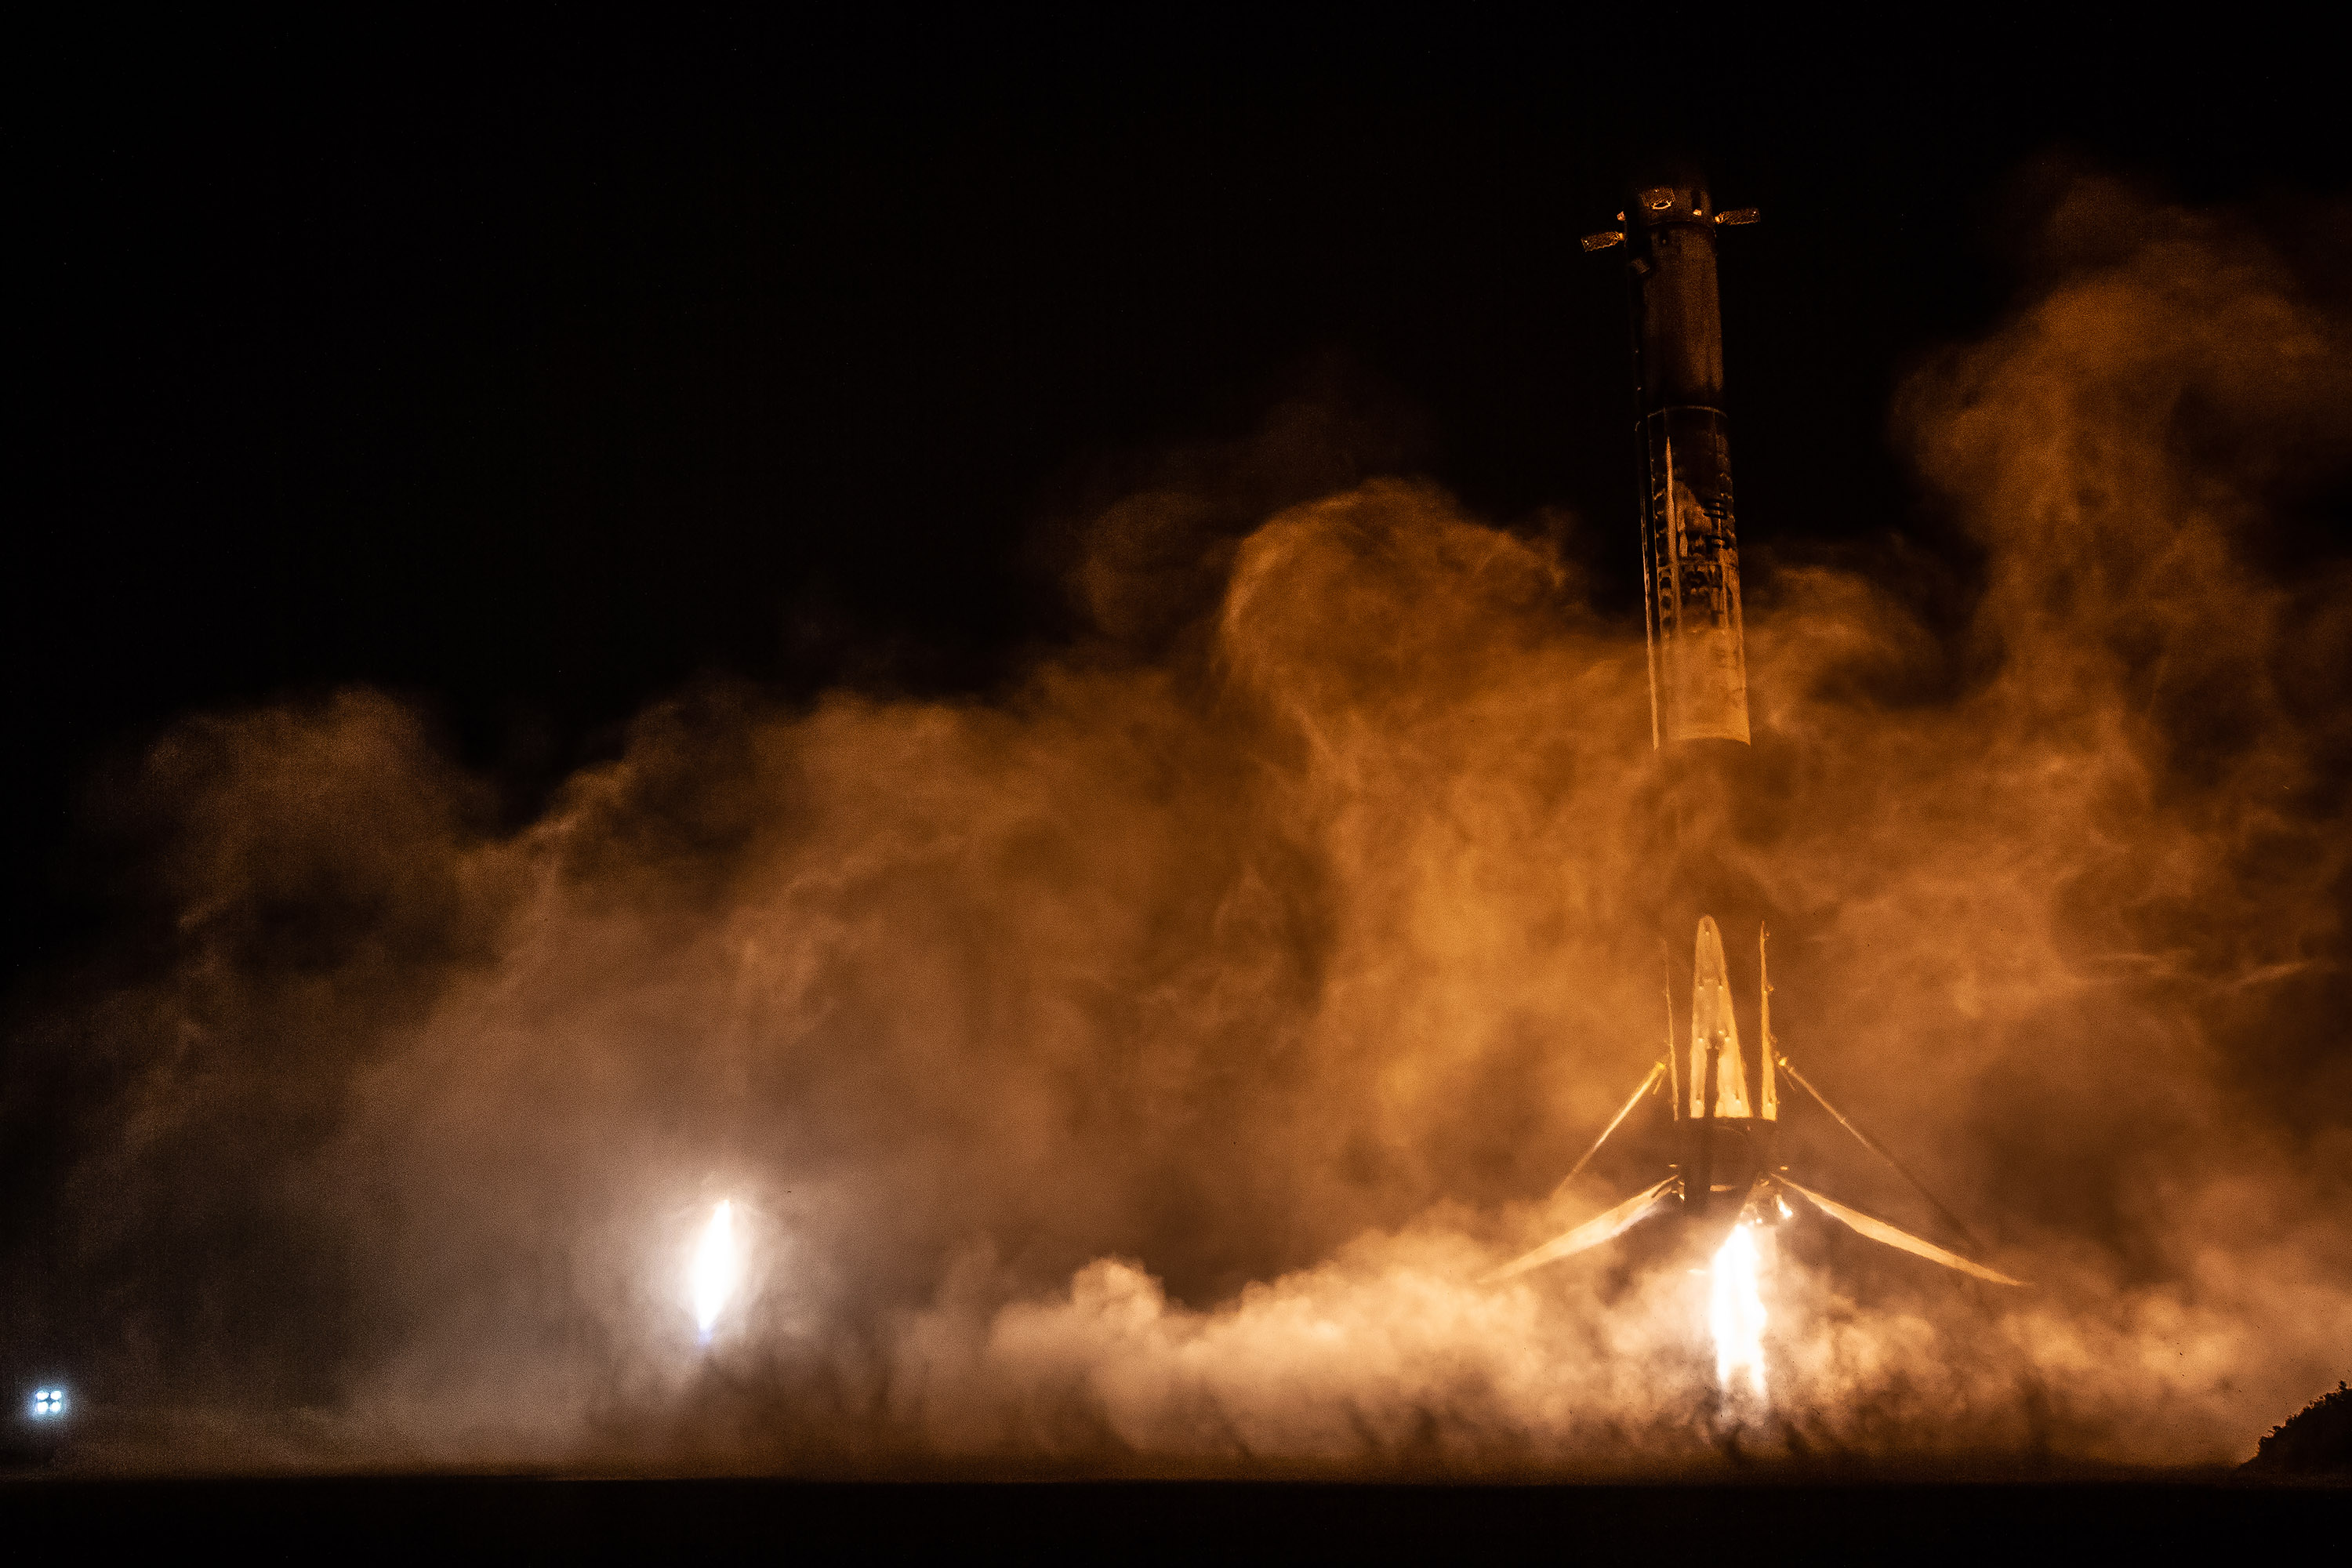
\includegraphics[%
      height = 9.5in,%
      trim = 300 20 0 50,
      clip%
    ]{images/STP-2-Mission-Landing}%
  };

  \node [at={($(current page.north west)+0.5*(1, 0)$)}] (A1) {};
  \node [at={($(current page.south west)+1.0*(1, 0)$)}] (A2) {};
  \node [at={($(current page.south west)+2.0*(0, 1)$)}] (B) {};
  \node [at={($(current page.south east)+0.5*(0, 1)$)}] (C) {};

  \fill [color={Orange}, path fading={fade lightly right}]
    (A1)
    rectangle
    (A2);

  \fill [color={RichBlack}]
    (current page.south west)
    rectangle
    (A1);
  \fill [color={RichBlack}]
    (current page.north west)
    --
    ($(current page.north west) + 1.0*(1, 0)$)
    --
    ($(current page.north west) - 1.0*(0, 1)$)
    --
    (current page.north west);
\end{tikzpicture}
\vfill
\begin{flushright}
{
  \rmfamily\HUGE\noindent
  \textbf{ECE 380 --- Intro to Feedback Control}\\
  Spring 2020\\
  {Lab Manual v0.4}\\
  {
    \scshape
    \small Built \today ---
    \makeatletter
    \small Commit {%
      \@@input|"git rev-list --max-count=1 HEAD | cut -c -6 -"
    }
    \makeatother
  }
}
\end{flushright}
\begin{flushright}
{
  \rmfamily\Large\noindent
  Rollen S. D'Souza
}
\end{flushright}
\vspace{0.25in}
\end{titlingpage}

\restoregeometry

\pagebreak
% END: TITLE PAGE
%%%%%%%%%%%%%%%%%%%%%%%%%%%%%%%%%%%%%%%%%%%%%%%%%%%%%%%%%%%%%%%%%%%%%%%%%%%%%%%

%%%%%%%%%%%%%%%%%%%%%%%%%%%%%%%%%%%%%%%%%%%%%%%%%%%%%%%%%%%%%%%%%%%%%%%%%%%%%%%
% BEG: COPYRIGHT BS
%
\thispagestyle{empty}
%\noindent\textcopyright 2020 Rollen S. D'Souza\\

\noindent
Cover page image captured by SpaceX\textregistered~on their
STP-2 Mission, licensed under the Creative Commons Non-Commercial 2.0. See
\href{https://www.flickr.com/photos/spacex/48129269942/}{here}
for original content. It is, of course, a photo of one of their self-landing
booster rockets attempting a landing. If you are interested, see the discussion
by Lars Blackmore on \emph{Autonomous Precision Landing of Space Rockets}
in
\href{http://www.larsblackmore.com/nae_bridge_2016.pdf}{this publication}. It
isn't very technical but you can find where to jump from there if you want a
little more technical content.
\begin{center}
  * \qquad * \qquad *
\end{center}
\noindent
A big thank you to
\begin{itemize}[label={}]
  \item{Carmen Caradima,}
  \item{Prof. Christopher Nielsen,}
  \item{Prof. Andrew Heunis,}
\end{itemize}
and other ECE 380 lab and course instructors whose work has inspired much
of this lab manual. This lab manual is just a variation of past
ECE 380 labs. Thank you to Prof. Derek Rayside whose general teaching
style inspires the variations made in this lab.
\begin{center}
  * \qquad * \qquad *
\end{center}

\pagebreak
% END: COPYRIGHT BS
%%%%%%%%%%%%%%%%%%%%%%%%%%%%%%%%%%%%%%%%%%%%%%%%%%%%%%%%%%%%%%%%%%%%%%%%%%%%%%%

\frontmatter

\tableofcontents*
\thispagestyle{empty}

\clearpage
\listoffigures*

\clearpage
\listoftables*

%%%%%%%%%%%%%%%%%%%%%%%%%%%%%%%%%%%%%%%%%%%%%%%%%%%%%%%%%%%%%%%%%%%%%%%%%%%%%%%
% BEG: INTRODUCTION
%
\chapter{Introduction}
Welcome to your remote lab for ECE 380, Introduction to Feedback Control.
The in-lab portion of this course was designed to give you a hands-on
feel for control using analog circuits. Given the current climate, this is
clearly not possible in the way previously envisioned.

We persist. This lab is designed to run in MATLAB and Simulink. You will engage
in understanding, developing, executing and analyzing Simulink
diagrams that model and simulate control systems. Every lab, though
somewhat artificial, is
provided with brief motivation on how one can see this applied in a real
world problem. I hope I can help connect the abstract block diagrams of
Simulink with the real world for you.

Control systems is a very broad topic with a long history that even predates
the ideas discussed in this course. This course and lab covers the very basic
notion of control, the idea of the negative feedback loop, buttressed by
the mathematical tools of linear dynamical systems.

\section{MATLAB and Simulink}
MATLAB is a desktop numerical and symbolic
mathematics computing environment. We will not rely heavily on MATLAB
scripting itself and instead use Simulink but you should be familiar with
both environments. Please ensure that, when you are installing MATLAB, you
install
%
\begin{enumerate}[label=(\arabic*)]
  \item{
    MATLAB,
  }
  \item{
    Simulink,
  }
  \item{
    the Control Systems Toolbox,
  }
  \item{
    the Simulink Control Design,
  }
  \item{
    the DSP System Toolbox,
  }
  \item{
    the Signal Processing Toolbox,
  }
  \item{
    the Statistics and Machine Learning Toolbox and
  }
  \item{
    the Symbolic Math Toolbox.
  }
\end{enumerate}
%
Simulink is an add-on to MATLAB that allows you to design and simulate
systems (physical or otherwise) using block diagrams like in
Figure~\ref{fig:intro:1}.
%
\begin{figure}
  \centering
  \begin{tikzpicture}[x=1in, y=1in]
    \node [draw, block] (Controller) {\(K_p + K_i\frac{1}{s}\)};
    \node [draw, block, right=0.5 of Controller] (Plant) {\(\frac{1}{s}\)};
    \node [draw, summer, left=0.5 of Controller] (Sum) {};
    \node [below=0.5 of Sum] (BelowSum) {};

    \draw [arrow, signal]
      (Controller.east) -- (Plant.west);
    \draw [arrow, signal]
      (Plant.east)
      --
      +(0.35, 0)
      |-
      (BelowSum.base)
      --
      (Sum.south)
      node [below right, annotate] {\(-\)};
    \draw [arrow, signal]
      (Sum.east) -- (Controller.west);
    \draw [arrow, signal]
      ($(Sum.west)+1*(-0.5, 0)$) -- (Sum.west);
    \draw [arrow, signal]
      (Plant.east) -- +(0.7, 0);
  \end{tikzpicture}
  \caption[Example Feedback Diagram]{
    Example feedback diagram. The blocks are differential equations, expressed
    as a Laplace transfer function, that take an input signal and produce an
    output signal.
  }
  \label{fig:intro:1}
\end{figure}
%
Figure~\ref{fig:intro:1} can be replicated perfectly in Simulink.
That fact makes it easy for engineers to quickly design and verify
control designs. Simulink even supports direct interaction with
hardware but we will not utilize this feature.

The core of Simulink is the notion of a \emph{block}, maps that take an input
signal and produce an output signal.
The blocks we'll be concerned with primarily are \emph{gains}
(multiplier) depicted in Simulink like
\begin{center}
  \begin{tikzpicture}[x=1em, y=1em]

    \draw
      (0, 0)
      --
      (3, 1)
      --
      (0, 2)
      --
      (0, 0)
      --
      (3, 1)
      node [at={(1, 1)}] {\(K\)};

  \end{tikzpicture}
\end{center}
and \emph{transfer functions} depicted in Simulink like
\begin{center}
  \begin{tikzpicture}[x=1em, y=1em]

    \node [draw, block] (Plant) {\(\frac{s+1}{s+2}\)};

  \end{tikzpicture}.
\end{center}
You may be provided template blocks to help you setup the Lab plant, the
system we wish to control; it will then be your task to analyze this block,
design a controller, and implement it by linking up blocks
in the appropriate feedback architecture.

% \section{Git Version Control}
% We will be using the \texttt{git} version control system in tandem with
% the Gitlab hosted on \url{git.uwaterloo.ca} to facilitate delivery of lab
% content and to give you a mechanism for
% \begin{enumerate}[label=(\arabic*)]
%   \item{tracking your temporary work, and}
%   \item{submitting your final work.}
% \end{enumerate}
% There is no requirement that you use git ``properly.'' If you are not
% comfortable using the terminal to perform git operations, you can use graphical
% tools like \href{https://www.sourcetreeapp.com/}{Sourcetree} or
% \href{https://www.gitkraken.com/git-client}{GitKraken}. You can even manually
% upload the files using the graphical web interface at \url{git.uwaterloo.ca}.
% As long as your able to download files from your repository and upload your
% solutions, I am happy. Having said that, it is an important skill in this
% day and age to understand how to use version control. This is a
% great opportunity to learn git!

\section{Lab Logistics and Deliverables}\label{intro:logistics}
Lab deadlines can be found in Table~\ref{tab:labcalendar}. Read carefully.
I have provided all times in both EDT as well as UTC.
Every lab requires you to complete a number of procedures described in
green boxes like
\begin{procedure}[]
  Here are some steps:
  \begin{enumerate}[label=(\arabic*)]
    \item{Yes here is step 1,}
    \item{oh wow step 2,}
    \item{really you are still reading this,}
    \item{you must be really bored,}
    \item{consider finding better things to do.}
  \end{enumerate}
\end{procedure}
\noindent
and deliverables described in red boxes like
\begin{deliverable}[]
  Here are some things you will need to save for your report.
\end{deliverable}
Procedures are simply steps you should follow that will eventually result in
a deliverable, which is something you must record and submit as part of your
report. Every lab chapter ends with a final summative deliverable, usually
consisting of a series of questions that you must answer.
%
All the deliverables should be packaged up in an organized way; ideally
they should be in your report in the order presented under headings directly
corresponding to the deliverable label (1.1, 1.2, etc.). Your final report
must be submitted as a PDF document on Learn. Your grade is entirely based
on your report. Every lab has its own grading scheme, but the following
penalties apply equally to all labs:
\begin{itemize}
  \item{
    \(-5\%\) for not having a typeset document or for poor organization,
  }
  \item{
    \(-10\%\) for not submitting a PDF,
  }
  \item{
    \(-20\%\) within the first \texttt{24} hours it is late. After
    \texttt{24} hours, it becomes \(-100\%.\) If prior arrangements are made
    or a valid reason presented within a week from the missed deadline, this
    is waived. In no case will a lab report be accepted more than a week past
    the deadline; if a valid reason exists for being unable to hand in the lab
    within the week following the deadline, then the lab will be assigned a
    weight of zero and the remaining labs will be reweighted accordingly.
    \textbf{Contact the Lab Instructor for this.}
    All reports are due at \texttt{23:59:59 EDT} on the due date.
    All deadlines will be reported both
    in Eastern Daylight Time (\texttt{EDT}) and Coordinated Universal Time
    (\texttt{UTC})
    so that there can be no confusion on the deadline in case you are not
    in Waterloo.
  }
\end{itemize}
%
In terms of general style, I am a proponent of letter grade style
grading schemes for discussion questions.
Often grading is arbitrary and it can be hard to really pin down the value of
a question especially when the content has no obvious discrete points to
get correctly for the student and marker. I will have markers
rate these discussion answers on the scale shown in
Figure~\ref{tab:letter-grading}.
%
\begin{table}
\centering
\begin{tabular}{r|c|l}
Value & Letter & Explanation\\ \hline
\(100\%\) & A+ & Meets Expectations.\\ \hline
\(90\%\)  & A & Meets Expectations. Answer could be Improved Upon. \\ \hline
\(80\%\) & B & Would Meet Expectations. Made Minor Mistakes.\\ \hline
\(60\%\) & C & Would Meet Expectations. Made a few Major Mistakes.\\ \hline
\(40\%\) & D & Fundamental Lack of Understanding in Attempt.\\ \hline
\(0\%\) & F & No Understanding or No Work Shown.
\end{tabular}
\caption[Letter Grading Scheme]{Letter grade with associated value and
description for how we assign the grade.}
\label{tab:letter-grading}
\end{table}
%
Minor mistakes are penalized quite steeply so check your work. Mistakes in
discussions usually amount to theoretical mistakes in understanding; empirical
mistakes are deducted in other rows and we will make an attempt to avoid double
(cascade) deductions. The letter grade \(A\) is reserved for when discussion
responses have no mistakes but a better explanation exists or an explanation
ought to be expanded upon. This is to prevent steep penalties for purely a
lack of insight.

%
\begin{table}
  \centering
  \begin{tabular}{c|c|c|l}
      & Release Date & Due Date & Grading Release Date\\ \hline
    Form Your
      &
      & \texttt{17 MAY 1159 EDT}
      & \\
    Group
      &
      & \texttt{18 MAY 0359 UTC}
      & \\ \hline
    Lab 1
      & \texttt{17 MAY 1159 EDT}
      & \texttt{24 MAY 1159 EDT}
      & {\color{blue}\texttt{31 MAY 1159 EDT}}\\
      & \texttt{18 MAY 0359 UTC}
      & \texttt{25 MAY 0359 UTC}
      & {\color{blue}\texttt{01 JUN 0359 UTC}}\\ \hline
    Lab 2
      & {\color{blue}\texttt{31 MAY 1159 EDT}}
      & {\color{blue}\texttt{07 JUN 1159 EDT}}
      & {\color{blue}\texttt{14 JUN 1159 EDT}}\\
      & {\color{blue}\texttt{01 JUN 0359 UTC}}
      & {\color{blue}\texttt{08 JUN 0359 UTC}}
      & {\color{blue}\texttt{15 JUN 0359 UTC}}\\ \hline
    Lab 3
      & {\color{blue}\texttt{14 JUN 1159 EDT}}
      & {\color{blue}\texttt{21 JUN 1159 EDT}}
      & {\color{blue}\texttt{28 JUN 1159 EDT}}\\
      & {\color{blue}\texttt{15 JUN 0359 UTC}}
      & {\color{blue}\texttt{22 JUN 0359 UTC}}
      & {\color{blue}\texttt{29 JUN 0359 UTC}}\\ \hline
    Lab 4
      & {\color{blue}\texttt{05 JUL 1159 EDT}}
      & {\color{blue}\texttt{12 JUL 1159 EDT}}
      & {\color{blue}\texttt{19 JUL 1159 EDT}}\\
      & {\color{blue}\texttt{06 JUL 0359 UTC}}
      & {\color{blue}\texttt{13 JUL 0359 UTC}}
      & {\color{blue}\texttt{20 JUL 0359 UTC}}\\ \hline
    Lab 5
      & {\color{blue}\texttt{26 JUL 1159 EDT}}
      & {\color{blue}\texttt{02 AUG 1159 EDT}}
      & {\color{blue}\texttt{09 AUG 1159 EDT}}\\
      & {\color{blue}\texttt{27 JUL 0359 UTC}}
      & {\color{blue}\texttt{03 AUG 0359 UTC}}
      & {\color{blue}\texttt{10 AUG 0359 UTC}}
  \end{tabular}
  \caption[Lab Calendar]{%
    Lab Calendar showing release dates, due dates and expected grading
    deadlines. Tentative dates are colored blue.
  }
  \label{tab:labcalendar}
\end{table}

% END: INTRODUCTION
%%%%%%%%%%%%%%%%%%%%%%%%%%%%%%%%%%%%%%%%%%%%%%%%%%%%%%%%%%%%%%%%%%%%%%%%%%%%%%%

\mainmatter
\chapter{System Identification Fundamentals}\label{Lab:1}
Low-pass filters are ubiquitous. They can be found in the hardware of
audio processing chips, or the software of image editing tools. As you may
recall from a course on Signals and Systems theory\footnote{If you haven't
taken a course in Signals and Systems, speak to your Lab Instructor on
knowledge you may be lacking.}, a low-pass filter
is a system that, generally speaking, rejects high-frequency signals while
``passing through'' low-frequency signals. In this lab you will be asked
to analyze a low-pass filter block and determine its parameters via a time
domain approach. This is not meant to be a difficult lab and is instead
designed to give you a sense of the lab format. However, it will put to the
test your knowledge of signals and systems. If you have forgotten your
Laplace transforms, this is a good time to remind yourself of them!

In the real world, our models are rarely perfect. The techniques
you learn here generalize nonetheless. Whenever you confront a novel system,
devise a generic model that you think characterizes its behaviour and then
come up with experiments that expose its characteristics; this gives you
estimates of the generic model's parameters that best fit the actual system.
We will encounter such a situation in a future lab.

\section{Objectives}
The primary objectives of this lab are to
\begin{enumerate}[label=(\arabic*)]
  \item{
    \textbf{Install} MATLAB, Simulink and required toolboxes.
    Alternatively, \textbf{connect remotely} to
    \url{engterm.uwaterloo.ca} or any other lab computer of your choice
    that has MATLAB.
  }
  \item{
    Understand how to \textbf{open} and \textbf{modify}
    a Simulink diagram and how to run a simulation.
  }
  \item{
    Understand how to \textbf{log} signals for future inspection.
  }
  \item{
    Understand how to \textbf{plot} figures and capture them.
  }
  \item{
    Understand the theory behind first-order low-pass systems.
  }
  \item{
    Understand how to \textbf{identify} a first-order low-pass system.
  }
\end{enumerate}
This is not a particularly long lab, but you may have trouble as it is
very likely your first encounter with Simulink. As a result, I suggest you
give you and your partner time to work through the lab and the problems.
I also recommend you spend some time by yourself exploring Simulink so as to
reduce the amount of time you spend on future labs.

\section{Experimental Procedure}
This entire lab will be done using the ``\texttt{Lab\_1.slx}'' Simulink model.
First extract the ``\texttt{Lab\_1\_Data.zip}'' file available from Learn.
Inside there you will find zip files created for each individual group. Extract
the zip file associated to your group, and there you will find the relevant
``\texttt{Lab\_1.slx}'' file. The R2018 version may be found in a nested
directory.

In the Simulink model you will
find a number of blocks already placed for you in an open loop configuration:
\begin{itemize}
  \item{a signal generator,}
  \item{a summing junction,}
  \item{an adjustable gain block,}
  \item{a ``plant'', the system we are going to analyze, and}
  \item{a terminator.}
\end{itemize}
%
The plant --- labelled \(P(s)\) in the diagram --- can be assumed to be a
transfer function taking the form
\[
  P(s) = \frac{b T}{s + a T} \quad ,
\]
where \(a, b > 0\) and \(T \in \{10, 100\}.\) Your goal is to use the
techniques described in the following subsections to estimate the parameters
\(a,\) \(b\) and \(T\) for your plant. This process is known as
\textbf{system identification} and it is a critical precursor to control
design. How can we design a controller if we don't even know the parameters
of the system we wish to control?

\subsection{Acquiring the Bandwidth in Time-Domain}
The goal of this portion of the lab is to acquire the bandwidth of the
given linear system. What is the bandwidth? To understand and acquire it,
we must first know what the DC gain of a system is.
%
\begin{definition}[label={def:lab1:dcgain}]{DC Gain}
  Let \(G(s)\) be a \emph{stable} transfer function
  that maps an input signal \(U(s)\) to an
  output \(Y(s).\) The \textbf{DC gain} of \(G(s)\) is \(G(0)\) and,
  if \(u(t) = A \mathbf{1}(t)\) for \(A \in \Real,\) it satisfies the relation
  \[
    \lim_{t\to \infty} y(t) = A G(0).
  \]
\end{definition}
%
Observe that the DC gain \(G(0)\) is called precisely that because when we
apply a square (DC-like; step) signal change, the system's output converges
to the amplitude of the input times \(G(0).\)
%
Instead of computing the DC gain by evaluating the system's response to a step
input, we take a different approach.
%
\begin{procedure}[label={proc:lab1:p1}]
  You will acquire the DC gain of the plant \(P(s)\). Follow these steps:
  \begin{enumerate}[label=(\arabic*)]
    \item{
      \textbf{Open} the signal generator block, \textbf{set} the type of signal
      to be a sinusoidal wave, and set the
      \textbf{amplitude} to be \(1\) and the \textbf{frequency}
      to be \(\SI{0.5}{Hz}.\) This signal is so low frequency that it
      emulates a constant signal. Note that any lower frequency than this will
      work just as well.
    }
    \item{
      \textbf{Run} the script \texttt{generate\_lab\_1\_plot.m} and inspect
      Figure 1, which depicts the input and output signal.
    }
    \item{
      \textbf{Measure the peak to peak amplitudes} of the input and output signals respectively when the system is in steady-state.
    }
    \item{
      \textbf{Estimate} the DC gain by dividing the output amplitude
      by the input amplitude. \emph{Remember, we chose the input amplitude
      to be \(1\)!}
    }
  \end{enumerate}
\end{procedure}
%
\begin{figure}
  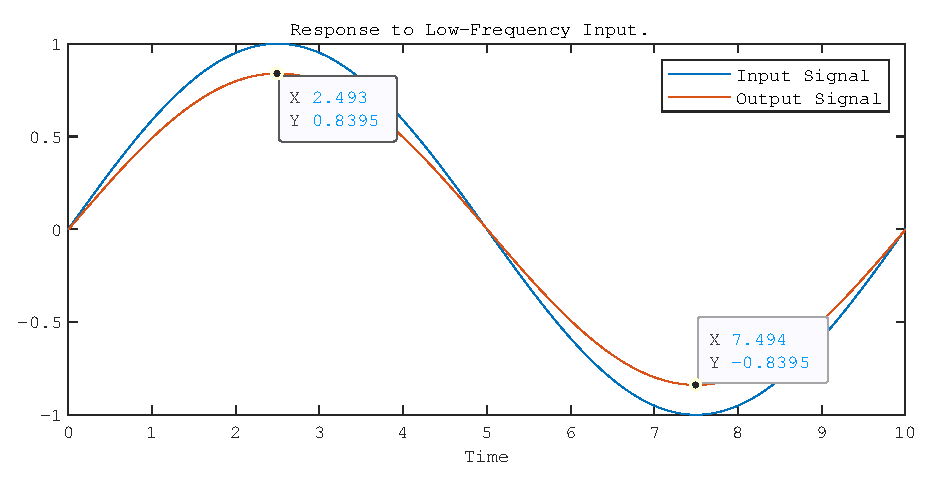
\includegraphics{images/Lab_1_LowFrequency.eps}
  \caption[Low Frequency Response of a Low-Pass Plant]{The low-frequency response to my low-pass plant \(P(s).\) The gain
  at this low frequency is \(0.8395.\) Can you see why? What is the DC
  gain approximately?}
  \label{fig:lab1:lowfreq}
\end{figure}
%
\begin{figure}
  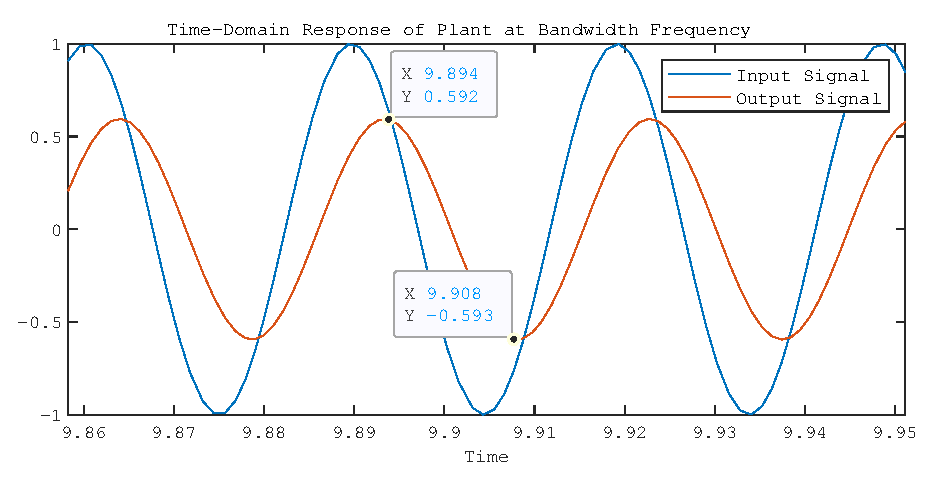
\includegraphics{images/Lab_1_Bandwidth.eps}
  \caption[Time-Domain Response of a First-Order System at the Bandwidth Frequency]{The response to my \(P(s)\) at the bandwidth frequency.
  Can you see why this is the bandwidth frequency for my plant?}
  \label{fig:lab1:bandwidth}
\end{figure}
%
\begin{deliverable}[label={lab1:d1}]
  \textbf{Record} your estimated DC gain and \textbf{capture} the generated
  figure with the cursors you used to measure the amplitudes.
  Your figure should like Figure~\ref{fig:lab1:lowfreq}.
\end{deliverable}
%
For low-pass systems, as we increase the frequency of the input, we will
observe, the output amplitude \emph{decreases}. The bandwidth frequency
is the frequency that marks the point where we distinguish between the
``low'' frequency inputs a low-pass system sustains and the ``high'' frequency
inputs a low-pass system rejects.
%
\begin{definition}[]{Bandwidth}
  Let \(G(s)\) be a proper transfer function
  that maps an input signal \(U(s)\) to an output \(Y(s).\)
%
  Say the input is a sinusoid of the form \(A \cos(\omega t)\) with amplitude
  \(A.\) In steady-state, the amplitude of \(y(t)\) converges to a constant
  \(B.\) The \textbf{gain at frequency \(\omega\)} is
  \(\left\|G(j\omega)\right\| = \frac{B}{A}.\)
%
  The \textbf{bandwidth (frequency)} of \(G(s)\) is the \emph{smallest}
  frequency \(\omega\) which satisfies
  \[
    \frac{1}{\sqrt{2}} = \frac{\left\|G(j\omega)\right\|}{\left\|G(0)\right\|}.
  \]
\end{definition}
%
What is the definition above trying to characterize? The
gain is the multiplier between the input amplitude and output amplitude. For
a low-pass system, this gain decreases as a function of input frequency. The
bandwidth frequency is the frequency where this gain has fallen, in comparison
to the DC gain, by factor of \(\sqrt{2}.\) This is further demonstrated
by the difference in response we observe between Figure~\ref{fig:lab1:lowfreq}
and Figure~\ref{fig:lab1:bandwidth}. Note how much smaller the output signal
is in the response with higher frequencies in comparison to the response
with lower frequencies.
%
\begin{procedure}[label={proc:lab1:p2}]
  You will acquire the bandwidth frequency of the plant \(P(s)\).
  Follow these steps:
  \begin{enumerate}[label=(\arabic*)]
    \item{
      \textbf{Predict} the amplitude of the steady-state output at the
      bandwidth frequency. As an example, if your DC gain is \(0.8395\) then
      the ratio between the input signal amplitude and the output signal
      at the bandwidth frequency is
      \[
        \frac{0.8395}{\sqrt{2}}.
      \]
      If my input signal has amplitude \(1,\) then I should look for
      an output signal amplitude with the above value.
    }
    \item{
      \label{lab1:p2:2}
      \textbf{Open} the signal generator block, \textbf{set} the type of signal
      to be a sinusoidal wave, and set the
      \textbf{amplitude} to be \(1\) and
      the \textbf{frequency} to be \(\SI{0.5}{Hz}.\)
    }
    \item{
      \textbf{Run} the script \texttt{generate\_lab\_1\_plot.m} and inspect
      Figure 1, which depicts the input and output signal.
    }
    \item{
      \label{lab1:p2:4}
      \textbf{Measure the amplitudes} of the output signal
      when the system is in steady-state.
    }
    \item{
      If the amplitude isn't what you want, repeat Steps~\ref{lab1:p2:2} through~\ref{lab1:p2:4} with a different frequency. Increase or decrease
      by orders of magnitude to speed up the process!
    }
    \item{
      If the amplitude is what you predicted, \textbf{record} the frequency
      of the input you used to achieve the result.
    }
  \end{enumerate}
\end{procedure}
%
\begin{deliverable}[label={lab1:d2}]
  At the bandwidth frequency,
  \textbf{capture a figure} of the input and output signal. It should look
  like Figure~\ref{fig:lab1:bandwidth}. Pay close attention to the time
  axis; it has been scaled to make the signal easy to measure and to visualize.
\end{deliverable}
%
Having acquired the bandwidth for the open loop system, we now investigate
the closed loop system.
%
\begin{figure}
  \centering
  \begin{tikzpicture}[x=1in, y=1in]
    \node [draw, block] (Controller) {\(K_p\)};
    \node [draw, block, right=0.5 of Controller] (Plant) {\(P(s)\)};
    \node [draw, summer, left=0.5 of Controller] (Sum) {};
    \node [below=0.5 of Sum] (BelowSum) {};

    \draw [arrow, signal]
      (Controller.east) -- (Plant.west)
      node [below left, annotate] {\(u\)};
    \draw [arrow, signal]
      (Plant.east)
      --
      +(0.35, 0)
      |-
      (BelowSum.base)
      --
      (Sum.south)
      node [below right, annotate] {\(-\)};
    \draw [arrow, signal]
      (Sum.east) -- (Controller.west);
    \draw [arrow, signal]
      ($(Sum.west)+1*(-0.5, 0)$) -- (Sum.west)
      node [below left, annotate] {\(r\)};
    \draw [arrow, signal]
      (Plant.east) -- +(0.7, 0)
      node [below, annotate] {\(y\)};
  \end{tikzpicture}
  \caption[Closed-Loop Diagram for Lab 1]{
    Closing the loop around the Plant \(P(s)\) for Lab 1.
  }
  \label{fig:lab1:closing-loop}
\end{figure}
%
\begin{procedure}[label={proc:lab1:p3}]
  Now \textbf{close the loop} around the slider gain and plant \(P(s).\) That
  is, connect your diagram so that it looks like Figure
  \ref{fig:lab1:closing-loop}. Then \textbf{set} the gain \(K_p\) to
  \(1.\)
  Repeat Procedures~\ref{proc:lab1:p1} and~\ref{proc:lab1:p2} for the
  closed-loop system depicted in Figure~\ref{fig:lab1:closing-loop}.
\end{procedure}
%
\begin{deliverable}[label={lab1:d3}]
  Repeat Deliverables~\ref{lab1:d1} and~\ref{lab1:d2} for the closed-loop
  system discussed in Procedure~\ref{proc:lab1:p3}
\end{deliverable}

\subsection{Acquiring the Settling Time and Time Constant}
In this section of Lab 1 we take a different approach to estimating the plant
parameters. Instead of feeding in a sinusoid of low and high frequency, we
acquire what is known as the \textbf{step response}. The step response of
a plant \(P(s)\) is the output \(Y(s) = P(s) U(s)\) when \(U(s)\) is the unit
step function, i.e. \(U(s) = \frac{1}{s}.\) In practice, we often feed
square waves.
%
There are two characteristic values we care about for a first-order step
response. The \(2\%\)-settling time and the time constant.
\begin{definition}[]{The \(2\%\)-Settling Time}
  For a plant \(P(s)\) and step input \(U(s) = \frac{1}{s},\)
  the \textbf{\(2\%\)-Settling Time} is the time \(T\) it takes for
  the output \(y(t)\) to reach within \(2\%\) of its final value and stay
  within that \(2\%\) margin for all future time \(t > T.\)
\end{definition}
%
\begin{figure}
  \centering
  \subfloat[Complete step response.\label{fig:lab1:settling-time:a}]{%
    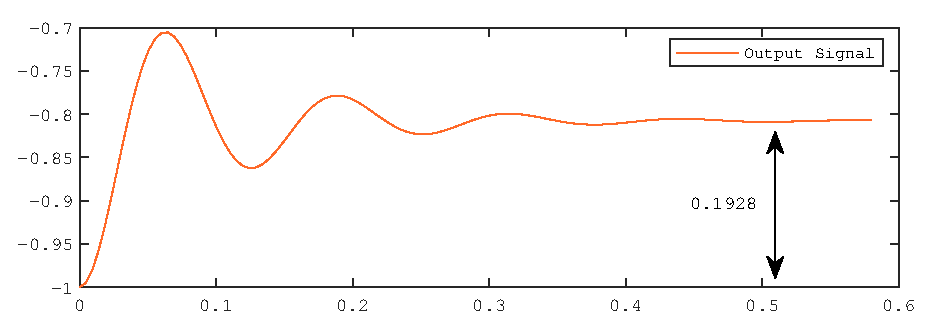
\includegraphics{images/Lab_1_SettlingTime_1.eps}%
  }\hfill
  \subfloat[Zoomed-in view on the settling behaviour of signal.%
  \label{fig:lab1:settling-time:b}]{%
    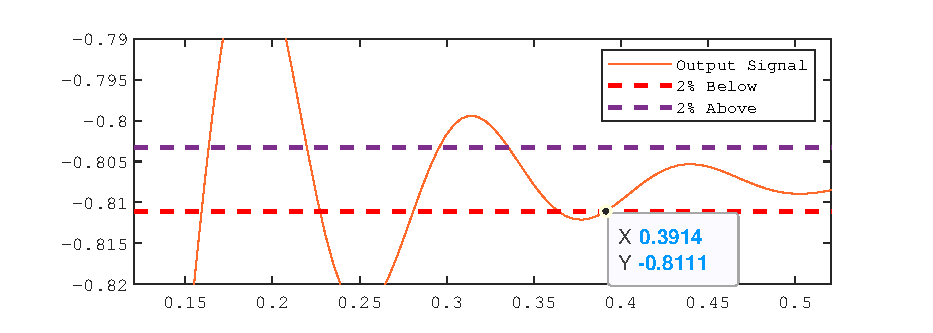
\includegraphics{images/Lab_1_SettlingTime_2.eps}%
  }
  \caption[Step Response for a Linear Plant depicting Settling Time Measurements]{
    The step response of some unknown plant with the \(2\%\)-settling time
    annotated in part (b). Observe how the the signal stays in
    the \(2\%\) region, demarcated by the broken lines,
    after the settling time of \(\SI{391.4}{ms}\) is attained.
  }
  \label{fig:lab1:settling-time}
\end{figure}
%
The settling time is a measure of long-term behaviour.
The notion is best depicted by Figure
\ref{fig:lab1:settling-time}.
In Figure~\ref{fig:lab1:settling-time:a} the ``net'' final value is
measured \emph{from the base to the top} of the signal. Then \(2\%\) of the
settling value is computed to define a cut-off point above and below the final
value, depicted as the broken lines in Figure
\ref{fig:lab1:settling-time:b}. Notice how the signal \emph{stays} in the
settling region after the settling time.
The next characteristic of the step response worthy of measurement is the
time constant. First let us define the standard first order form for a first
order transfer function.
%
\begin{definition}[]{Standard First-Order Form}
  The standard first order form for a strictly proper, first-order transfer
  function \(P(s)\) is
  \[
    P(s) = \frac{K}{\tau s + 1},
  \]
  where \(\tau, K \in \Real.\) The number \(\tau\) is called the \textbf{time
  constant}.
\end{definition}
%
It can be verified that the number \(K\) in the standard first order form
is simply the DC gain. The time constant can be estimated experimentally
in an easy way.
%
\begin{definition}[]{The Time Constant}
  For a first order plant \(P(s)\) and step input \(U(s) = \frac{1}{s},\)
  the time constant is the time \(\tau > 0\) it takes for
  the output \(y(t)\) to reach \(1-e^{-1} \approx 63\%\) of its final value.
\end{definition}
%
The time constant is a measure of transient, short-term behaviour. Note that,
unlike the settling time, the time constant only has meaning for a
first-order system. You will derive the relationship as one of your
deliverables.
%
\begin{procedure}[label={proc:lab1:p4}]
  In this procedure you will acquire the settling time and time constant
  of your plant \(P(s).\) First, \textbf{ensure} your plant is in open-loop
  configuration.
  \begin{enumerate}[label=(\arabic*)]
    \item{
      \textbf{Open} the signal generator block and \textbf{set} the type
      to be a square wave. Also, \textbf{set} the frequency to a low value,
      such as \(\SI{0.5}{Hz}.\) You will want to see atleast one step in
      the simulation but not too many more than that.
    }
    \item{
      \textbf{Run} the script \texttt{generate\_lab\_1\_plot.m} and inspect
      Figure 1, which depicts the input and output signal.
    }
    \item{
      Using cursors, \textbf{measure} the ``net'' final value by measuring from
      \emph{the base value of the signal to the final value}.
    }
    \item{
      Using the above measurement, \textbf{calculate} the \(63\%\) point
      where the time constant is found and \textbf{calculate} the \(2\%\)
      margins where the settling time is found.
    }
    \item{
      Using cursors, \textbf{measure} the time constant and settling times.
    }
  \end{enumerate}
\end{procedure}
%
\begin{deliverable}[label={lab1:d4}]
  \textbf{Capture the figure} you used to measure the settling time and
  time constant in Procedure~\ref{proc:lab1:p4}. \textbf{Show} your cursors.
\end{deliverable}
%
\begin{procedure}[label={proc:lab1:p5}]
  Repeat Procedure~\ref{proc:lab1:p4} for the closed-loop system described in
  Procedure~\ref{proc:lab1:p3}.
\end{procedure}
%
\begin{deliverable}[label={lab1:d5}]
  \textbf{Capture the figure} you used to measure the settling time and
  time constant in Procedure~\ref{proc:lab1:p5}. \textbf{Show} your cursors.
\end{deliverable}
%

\subsection{On Saturation or Clipping}
In practice, unlike in simulation, the signals we can apply to a system are
limited. This may be an inherent limitation, e.g.
power supply limitations, or a self-imposed safety limitation, e.g.
the angular velocity of an autonomous vehicle. Understanding where these hard
constraints appear in your control system is important, as usually these
constraints have \emph{nonlinear} effects! Ideally, we want to remain in
the region which has linear behaviour.

The only type of constraint you will encounter in these labs is the saturator
constraint. A \textbf{saturator}, or \textbf{clipper} as it is known in
electronics, limits a signal's maximum and minimum value to some preset
constant. In this section, you will attempt to find this limit.
%
\begin{procedure}[label={proc:lab1:p6}]
  \textbf{Put} your system in open-loop. \textbf{Set} the signal generator to
  generate a sinusoid with amplitude \(1\) at a low frequency.
  \textbf{Set} the gain \(K_p\) to \(1\) and \textbf{simulate}.
  \textbf{Increase} the gain \(K_p\) and \textbf{simulate} until you can
  observe the effects of saturation.
\end{procedure}
%
\begin{deliverable}[label={lab1:d6}]
  \textbf{Capture} the figure depicting the effects of saturation.
  \textbf{Record} the value of \(K_p\) where you had clipping occur.
\end{deliverable}

\section{Report Deliverable}
Good job! You made it through Lab 1. You are required to submit a report
that verifies you completed Lab 1 and that you understand the procedures you
performed. In addition to including
\begin{itemize}
  \item{Deliverable~\ref{lab1:d1},}
  \item{Deliverable~\ref{lab1:d2},}
  \item{Deliverable~\ref{lab1:d3},}
  \item{Deliverable~\ref{lab1:d4},}
  \item{Deliverable~\ref{lab1:d5} and}
  \item{Deliverable~\ref{lab1:d6}}
\end{itemize}
in your report,
you are required to answer the questions of the following deliverable.
Make sure to leverage your other deliverables in your answers!
\begin{deliverable}[label={lab1:report}]
  \begin{enumerate}[label={(\arabic*)}]
    \item{
      \label{lab1:report:q1}
      \textbf{Derive} a formula for the DC gain of \(P(s)\) in terms of
      \(a, b, T.\)
      \emph{Hint: Recall that the DC gain for a stable system \(G(s)\)
      is just \(G(0).\)}
    }
    \item{
      \label{lab1:report:q2}
      You know that your plant takes the form
      \[
        P(s) = \frac{b T}{s + a T}\quad ,
      \]
      for \(a, b > 0\) and \(T \in \{10, 100\}.\) \textbf{Derive} a
      formula for the bandwidth of \(P(s)\) in terms of \(a, b, T.\)
      \emph{Hint: Remember that the bandwidth frequency \(\omega\) solves
      the equation}
      \[
        \frac{\left\|P(j \omega)\right\|}{\left\|P(0)\right\|}
        =
        \frac{1}{\sqrt{2}}.
      \]
      \emph{Solve the expression for \(\omega.\) As
      an additional hint, you should get a polynomial in \(\omega^2\) which
      you can solve.}
    }
    \item{
      \label{lab1:report:q3}
      Using the formulas you derived in~\ref{lab1:report:q1} and
      \ref{lab1:report:q2} and the estimates of your bandwidth and DC gain
      in Procedures~\ref{proc:lab1:p1} and~\ref{proc:lab1:p2},
      \textbf{estimate} \(a, b, T.\) Recall that \(T\) can only take on
      values \(10\) or \(100.\)
    }
    \item{
      \label{lab1:report:q4}
      \textbf{Compare} the estimates of \(a, b, T\) made in
      \ref{lab1:report:q3} to your actual parameters.
      \textbf{Open} the ``\texttt{Lab\_1\_Data.sldd}'' to see your plant
      parameters. If there are discrepencies, explain why.
    }
    \item{
      \label{lab1:report:q5}
      \textbf{Find} a formula for the time constant of \(P(s)\) in terms of
      \(a, b, T.\) \emph{Hint: If you put \(P(s)\) in standard first order
      form, can you see what the time constant is?}
    }
    \item{
      \label{lab1:report:q6}
      \textbf{Find} the formula for the \(2\%\) settling time of \(P(s)\) in terms of \(a, b, T.\)
      \emph{Hint: You know \(P(s),\) the input \(U(s) = \frac{1}{s}\) and that
      the output is}
      \[
        Y(s) = P(s) U(s).
      \]
      \emph{Solve for an explicit expression for \(y(t)\) in the time domain.
      Then find how long it takes to reach \(2\%\) of the DC gain (the steady
      state value for a unit step)}
    }
    \item{
      \label{lab1:report:q7}
      Using the formulas you derived in~\ref{lab1:report:q5} and
      \ref{lab1:report:q6} and the estimates of the ``net'' final value (the signal in steady state), settling time and time constant in Procedure~\ref{proc:lab1:p4},
      \textbf{estimate} \(a, b, T.\)
    }
    \item{
      \label{lab1:report:q8}
      \textbf{Compare} the estimates of \(a, b, T\) made in
      \ref{lab1:report:q7} to your actual parameters.
    }
    \item{
      \label{lab1:report:q9}
      \textbf{Find} the transfer
      function from the input to the output when the system is in
      closed-loop, treating \(a, b, T, K_p\) as just unknown parameters.
      \emph{Hint: In closed loop you can write the input to the plant as
      \(U(s) = K_p(R(s) - Y(s))\)
      where \(R(s)\) is the input to the loop summing junction. See
      Figure~\ref{fig:lab1:closing-loop}. Combine this with \(Y(s) = P(s)U(s)\)
      and isolate \(Y(s)\) to get an expression \(Y(s) = G(s) R(s)\) where
      \(G(s)\) is some transfer function. Put \(G(s)\) in standard first order form.}
    }
    \item{
      \label{lab1:report:q10}
      \textbf{Discuss} how closing the loop, in Procedure
      \ref{proc:lab1:p3}, affected the bandwidth and DC gain.
      \textbf{Justify} your answer using the transfer function
      found in~\ref{lab1:report:q9}.
    }
    \item{
      \label{lab1:report:q11}
      \textbf{Discuss} how closing the loop, in Procedure
      \ref{proc:lab1:p5}, affected the settling time and time constant.
      \textbf{Justify} your answer using the transfer function
      found in~\ref{lab1:report:q9}.
    }
    \item{
      \label{lab1:report:q12}
      \textbf{Discuss} why we want to know the saturator limits. What would
      happen if we performed control design without verifying our control
      stayed within limits?
    }
  \end{enumerate}
\end{deliverable}

\subsection{Grading Scheme}
The grading scheme is shown in Table~\ref{tab:lab1:grading}. The breakdown of
your grade is shown per deliverable except in the case of the lab
questions where it is shown per question.
%
\begin{table}
\centering
\begin{tabular}{c|l|c}
        & Deliverable           & Marks  \\ \hline
        & \ref{lab1:d1}         & 2       \\ \hline
        & \ref{lab1:d2}         & 2       \\ \hline
        & \ref{lab1:d3}         & 2       \\ \hline
        & \ref{lab1:d4}         & 2       \\ \hline
        & \ref{lab1:d5}         & 2       \\ \hline
        & \ref{lab1:d6}         & 2       \\ \hhline{=|=|=}
Lab Subtotal&                       & 12      \\ \hhline{=|=|=}
        & \ref{lab1:report}~\ref{lab1:report:q1}  & 1       \\ \hline
        & \ref{lab1:report}~\ref{lab1:report:q2}  & 1       \\ \hline
        & \ref{lab1:report}~\ref{lab1:report:q3}  & 3       \\ \hline
        & \ref{lab1:report}~\ref{lab1:report:q4}  & 3       \\ \hline
        & \ref{lab1:report}~\ref{lab1:report:q5}  & 1       \\ \hline
        & \ref{lab1:report}~\ref{lab1:report:q6}  & 1       \\ \hline
        & \ref{lab1:report}~\ref{lab1:report:q7}  & 3       \\ \hline
        & \ref{lab1:report}~\ref{lab1:report:q8}  & 3       \\ \hline
        & \ref{lab1:report}~\ref{lab1:report:q9}  & 1       \\ \hline
        & \ref{lab1:report}~\ref{lab1:report:q10} & 5       \\ \hline
        & \ref{lab1:report}~\ref{lab1:report:q11} & 5       \\ \hline
        & \ref{lab1:report}~\ref{lab1:report:q12} & 1       \\ \hhline{=|=|=}
Report Subtotal&  & 28 \\ \hhline{=|=|=}
  Total &                       & 40
\end{tabular}
\caption[Grading Scheme for Lab 1]{Grading scheme for Lab 1.}
\label{tab:lab1:grading}
\end{table}
%

\chapter{Second-Order System Identification and Analysis}\label{Lab:2}
A large majority of systems we wish to control are physical systems. These
systems are often modelled using Newton's laws
\[
\begin{aligned}
  \mathrm{mass}~\frac{\mathrm d^2}{\mathrm{d}t^2}~\mathrm{position}
    &= \sum \mathrm{natural~forces} + \mathrm{applied~force},\\
  \mathrm{inertia}~\frac{\mathrm d^2}{\mathrm{d}t^2}~\mathrm{orientation}
    &= \sum \mathrm{natural~torques} + \mathrm{applied~torque},
\end{aligned}
\]
These systems --- when
they are linear --- result in second-order transfer functions from the
applied input (forces or torques) to the output (position and orientation).
It follows that if we want to understand how to effectively control physical
systems then we must first understand second-order systems and their
properties!

In this lab you will explore the generic characteristics of a second-order
linear system. You will discover the limitations of proportional error
feedback control --- the most na\'ive of control laws --- when applied to
a physical system. This motivates consideration of
more complicated control strategies. Labs 4 and 5 will explore these options.

\emph{A word of caution. This is the final lab where it is possible to
to find out the parameters of your system by inspecting the data file.
This, in principal, allows you to back-calculate what your procedures should
tell you. This was intentional to allow
you to check your work and ensure you understand how to perform the procedure.
However, future labs will assume you've perfected this procedure.
The parameters will be fairly well hidden like how it is sometimes in the
\texttt{\#RealWorld}. So, make sure you understand how to perform the
procedures!}

\section{Objectives}
The primary objectives of this lab are to
\begin{enumerate}[label=(\arabic*)]
  \item{
    \textbf{Learn} the characteristic properties of a standard second-order linear system.
  }
  \item{
    \textbf{Identify} the parameters of a standard second-order linear system.
  }
  \item{
    \textbf{Learn} how to acquire a Bode plot, the frequency response,
    and \textbf{understand} how to interpret it.
  }
  \item{
    \textbf{Explore} how a proportional control feedback affects the response
    of a second-order system.
  }
\end{enumerate}
Below is a dependency graph depicting the relationships between each of the
deliverables. If an arrow flows from A to B, that means B depends on the
partial or full completion of A.
\begin{center}
\begin{tikzpicture}[x=1em, y=1em]
  \node[deliverable] (D_2_1) {Deliverable\\\ref{lab2:d1}};
  \node[deliverable, below = 3em of D_2_1] (D_2_3) {%
    Deliverable\\\ref{lab2:d2b}%
  };
  \node[deliverable, right = 3em of D_2_3] (D_2_2) {%
    Deliverable\\\ref{lab2:d2}%
  };
  \node[deliverable, right = 3em of D_2_2] (D_2_7_4) {%
    Deliverable\\\ref{lab2:report}~\ref{lab2:report:q4}-\ref{lab2:report:q4b}%
  };
  \node[deliverable, at=(D_2_1-|D_2_7_4)] (D_2_7_1) {%
    Deliverable\\\ref{lab2:report}~\ref{lab2:report:q1}--\ref{lab2:report:q3}%
  };

  \node[deliverable, below = 3em of D_2_3] (D_2_4) {%
    Deliverable\\\ref{lab2:d3a}%
  };
  \node[deliverable, at = (D_2_4-|D_2_7_4)] (D_2_7_6) {%
    Deliverable\\\ref{lab2:report}~\ref{lab2:report:q5}%
  };
  \node[deliverable, below = 3em of D_2_4] (D_2_5) {%
    Deliverable\\\ref{lab2:d3}%
  };
  \node[deliverable, right = 6em of D_2_5] (D_2_6) {%
    Deliverable\\\ref{lab2:d4}%
  };
  \node[deliverable, right = 6em of D_2_6] (D_2_7_7) {%
    Deliverable\\\ref{lab2:report}~\ref{lab2:report:q6}%
  };
  \node[deliverable, below = 3em of D_2_7_7] (D_2_7_8) {%
    Deliverable\\\ref{lab2:report}~\ref{lab2:report:q8}%
  };


%  \draw[signal, arrow] (D_2_1.south) -- (D_2_3.north);
  \draw[signal, arrow] (D_2_1.east) -- (D_2_7_1.west);
  \draw[signal, arrow] (D_2_3.east) -- (D_2_2.west);
  \draw[signal, arrow] (D_2_2.east) -- (D_2_7_4.west);
  \draw[signal, arrow] (D_2_7_1.south) -- (D_2_7_4.north);
  \draw[signal, arrow] (D_2_4.east) -- (D_2_7_6.west);
  \draw[signal, arrow] (D_2_5.east) -- (D_2_6.west);
  \draw[signal, arrow] (D_2_5.east) -- (D_2_7_6.west);
  \draw[signal, arrow] (D_2_6.east) -- (D_2_7_7.west);

\end{tikzpicture}
\end{center}

\section{Experimental Procedure}
This entire lab will be done using the ``\texttt{Lab\_2.slx}'' Simulink model.
In there you will
find a number of blocks already placed for you in an open loop configuration:
\begin{itemize}
  \item{a step input,}
  \item{a summing junction,}
  \item{an adjustable gain block,}
  \item{a ``fill-in'', zero disturbance block,}
  \item{a ``plant'', the system we are going to analyze, and}
  \item{a terminator.}
\end{itemize}
This time we will \emph{not} use the signal generator and instead leverage
the Model Linearizer App. Its usage is described in Appendix
\ref{App:Simulink:ModelLinearizer}. You may acquire the step response
using the techniques described in Lab~\ref{Lab:1} but to acquire the frequency
response you will have to use the Model Linearizer app. In future, we will
primarily rely on the Model Linearizer app as it'll
unify all your data collection
requirements and is far easier to use than modifying a script and turning
on/off logging. For this lab, the input signal starts off configured
as \(r\) and the output signal as \(y.\) You will have to change it later
in the lab.
%
The plant --- labelled \(P(s)\) in the Simulink diagram --- can be assumed
to be a transfer function taking the form
\[
  P(s) = \frac{\hat{K}\omega_n^2}{s^2 + 2\zeta\omega_n s + \omega_n^2}.
\]
This form has a special name.
%
\begin{definition}[]{Standard Second-Order Form}
  The standard second-order order form for a strictly proper, second-order
  transfer function \(P(s)\) with no zero is
  \[
    P(s) = \frac{\hat{K} \omega^2}{s^2 + 2 \zeta \omega s + \omega^2}.
  \]
  where \(\omega\) is called the \textbf{natural frequency} and
  \(\zeta\) is the \textbf{damping ratio}.
\end{definition}
%
The primary goal of this experiment is to (1) estimate \(\zeta,\)\(\omega_n,\)
and \(\hat{K},\) (2) explore the characteristics of your system and
(3) see how the characteristics change under a proportional error controller.
When analyzing the \emph{closed loop system}, we put our system in the form
depicted by Figure~\ref{fig:lab2:closing-loop}.
%
\begin{figure}
  \centering
  \begin{tikzpicture}[x=1in, y=1in]
    \node [draw, block] (Controller) {\(K_p\)};
    \node [draw, block, right=0.5 of Controller] (Plant) {\(P(s)\)};
    \node [draw, summer, left=0.5 of Controller] (Sum) {};
    \node [draw, summer, right=0.5 of Plant] (DistSum) {};
    \node [above=0.5 of DistSum] (AboveDistSum) {};
    \node [below=0.5 of Sum] (BelowSum) {};

    \draw [arrow, signal]
      (AboveDistSum.base)
      --
      (DistSum.north)
      node [above right, annotate] {\(d\)};
    \draw [arrow, signal]
      (Controller.east) -- (Plant.west)
      node [below left, annotate] {\(u\)};
    \draw [arrow, signal]
      (Plant.east)
      --
      (DistSum.west)
      node [below left, annotate] {\(+\)};
    \draw [arrow, signal]
      (DistSum.east)
      --
      +(0.5, 0)
      |-
      (BelowSum.base)
      --
      (Sum.south)
      node [below right, annotate] {\(-\)};
    \draw [arrow, signal]
      (Sum.east) -- (Controller.west);
    \draw [arrow, signal]
      ($(Sum.west)+1*(-0.5, 0)$) -- (Sum.west)
      node [below left, annotate] {\(r\)};
    \draw [arrow, signal]
      (DistSum.east) -- +(1, 0)
      node [below, annotate] {\(y\)};
  \end{tikzpicture}
  \caption{
    Closing the loop around the Plant \(P(s)\) for Lab 2. Note that the
    loop is closed \emph{after} the disturbance has been added to the output.
  }
  \label{fig:lab2:closing-loop}
\end{figure}
%

\subsection{Measuring the Characteristics of a Second Order System}
In Lab~\ref{Lab:1}, you learned about the DC gain, the bandwidth, and
settling time of a first-order system.
We will use these characteristics, as well as one more new one, to help
characterize a second order plant.
%
Your deliverable for this section is
%
\begin{deliverable}[label={lab2:d1}]
  \textbf{Capture a figure} showing your system's open loop step response.
  \textbf{Measure} and \textbf{record}
  \begin{enumerate}[label=(\arabic*)]
    \item{the steady-state value \(y_{\mathrm{ss}},\)}
    \item{
      the time-to-peak value \(T_{\mathrm{peak}}\) and
      the peak value \(y_{\mathrm{max}},\) and
    }
    \item{
      the \(2\%\) settling time \(T_{\mathrm{s}}.\)
    }
  \end{enumerate}
  The figure included in your report must have \textbf{cursors} at the peak
  value and steady-state value.
\end{deliverable}
%
You are already familiar with most of these measurements. The new measurements
are the peak related measurements. For us, the following definition suffices.
%
\begin{definition}[]{Time-To-Peak and Overshoot}
  Let \(G(s)\) be a proper, stable transfer function
  that maps an input signal \(u(t)\) to an output \(y(t).\)
%
  Let \(u(t)\) be the (not necessarily unit) step function. The peak value
  of \(y(t)\) is the maximum value \(y(t)\) obtains, mathematically expressed
  by\footnote{normally \(\sup\) is used but this suffices for our purposes.}
  \[
    y_\mathrm{max} \defineas \max_{\tau \in \Real} \left| y(\tau) \right|
  \]
  and the time it obtains the peak value, known as \textbf{time-to-peak}
  is defined as
  \[
    T_\mathrm{peak} \defineas \argmax_{\tau \in \Real} \left| y(\tau) \right|.
  \]
  Then, if \(y_\mathrm{ss}\) is the steady-state value of \(y(t),\) the
  \textbf{percent overshoot} is defined as
  \[
    \%\mathrm{OS}
      \defineas
        \frac{%
          \left|
            \left|y_\mathrm{max}\right| - \left|y_\mathrm{ss}\right|
          \right|%
        }{%
          \left| y_\mathrm{ss}\right|%
        }.
  \]
\end{definition}
%
Figure~\ref{fig:lab2:peak} depicts the measurements you perform to acquire
the percent overshoot. You measure the maximum value of the output
signal and the steady-state value of the signal. Then you
compute the relative error between the maximum value and the settling value of
the output.
%
\begin{figure}
  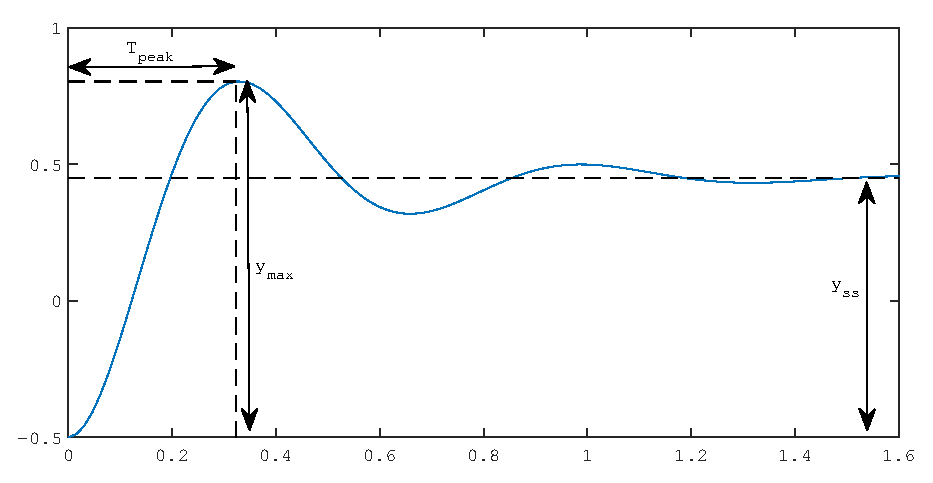
\includegraphics{images/Lab_2_Peak.eps}
  \caption[Depicting Overshoot Measurements for a Second-Order System.]{%
    The maximum peak occurs at time \(T_\mathrm{peak}\) with amplitude
    \(y_\mathrm{max}.\) The steady-state value is shown as \(y_{\mathrm{ss}}.\)
  }
  \label{fig:lab2:peak}
\end{figure}
%
\begin{procedure}[label={proc:lab2:p1}]
  In this procedure you will capture a variety of characteristics of
  your provided second-order system to achieve the goal of Deliverable
  \ref{lab2:d1} and to eventually characterize the parameters \(a,\)\(b\)
  and \(K.\)
  \begin{enumerate}[label=(\arabic*)]
    \item{
      \textbf{Ensure} your system is in the open loop configuration.
    }
    \item{
      \textbf{Ensure} that you indicate the signal before the summing junction
      is an input signal (Input Perturbation) and the signal after the plant
      is indicated as an output signal (Output Measurement). Refer
      to Appendix~\ref{App:Simulink:ModelLinearizer:2} for more information
      on how to do so.
    }
    \item{
      \textbf{Open} the Model Linearizer app and \textbf{capture} a
      step response. Refer to Appendix~\ref{App:Simulink:ModelLinearizer:3}
      on how to do so.
    }
    \item{
      \textbf{Measure} and \textbf{record} the following parameters of the
      output signal:
      \begin{itemize}
        \item{
          the steady-state value \(y_{\mathrm{ss}},\)
        }
        \item{
          the time-to-peak value \(T_{\mathrm{peak}}\) and
          the peak value \(y_{\mathrm{max}},\)
        }
        \item{
          the \(2\%\) settling time \(T_{\mathrm{s}}.\)
        }
      \end{itemize}
      \label{proc:lab2:p1:4}
    }
  \end{enumerate}
\end{procedure}

\subsection{Exploring Proportional Error Feeedback}
For this section you will explore how proportional error feedback affects
the behaviour of a second-order system. You will complete the following
deliverables.
%
\begin{deliverable}[label={lab2:d2}]
  \textbf{Capture} a single step response of your closed-loop system
  with a gain \(K_p \neq 1.\)
\end{deliverable}
%
\begin{deliverable}[label={lab2:d2b}]
  \textbf{Fill} three rows of the table
  \begin{center}
  \begin{tabular}{c|c|c|c|c}
    \(K_p\)
      & \(y_\mathrm{ss}\)
      & \(y_\mathrm{max}\)
      & \(T_\mathrm{peak}\)
      & \(\%\mathrm{OS}\) \\
    Gain
      & Steady-State Value
      & Peak Value
      & Time-To-Peak
      & Overshoot \\ \hline
    \(1\) & & & & \\ \hline
    Any & & & & \\ \hline
    Any & & & & \\ \hline
    & & & &
  \end{tabular}
  \end{center}
  for the closed loop system.
  Note that the overshoot is computed from \(y_\mathrm{ss}\) and
  \(y_\mathrm{max}.\)
\end{deliverable}

%
\begin{procedure}[label={proc:lab2:p2}]
  In this procedure you will explore a variety of gains \(K_p.\)
  \begin{enumerate}[label=(\arabic*)]
    \item{
      \textbf{Ensure} your system is in the closed-loop configuration
      as depicted in Figure~\ref{fig:lab2:closing-loop}.
    }
    \item{
      Choose a sequence of three gains to test. One of these gains
      must be \(K_p = 1.\) You may choose any value that is allowed by
      the slider gain provided to you in the Simulink Diagram.
    }
    \item{
      For each of your chosen gains \(K_p,\) \textbf{compute} the step
      response and \textbf{fill} the relevant row of the table
      in Deliverable~\ref{lab2:d2b}
    }
  \end{enumerate}
\end{procedure}

\subsection{Acquiring the Bandwidth in the Frequency-Domain}
Once again we will acquire the bandwidth of our system. We will do so for
\emph{both} the closed and open loop configurations. This time, however,
we will do so using the frequency response. In particular, you are asked
to complete the following deliverables.
%
\begin{deliverable}[label={lab2:d3a}]
  \textbf{Capture} a figure of the Bode plot for the open loop system.
  \textbf{Include} a cursor at the bandwidth frequency on the magnitude
  plot and a cursor where you estimated the DC gain.
\end{deliverable}
%
\begin{deliverable}[label={lab2:d3}]
  \textbf{Capture} a figure of the Bode plot for the closed loop system
  with unity gain (\(K_p = 1\)).
  \textbf{Include} a cursor at the bandwidth frequency on the magnitude
  plot.
\end{deliverable}
%
First of all, let us briefly review what a Bode plot depicts.
Given a \emph{real, rational and stable} transfer function \(G(s)\) and
(co)sinusoidal input
\(U(s) = \frac{s}{s^2 +\omega^2}\) of frequency \(\omega,\) the
output \(y(t)\) converges towards the signal
\[
  y_\mathrm{ss}(t)
    = \left\| G(j\omega) \right\| \cos(\omega t + \measuredangle G(j\omega)).
\]
Sometimes we say that the signal \(y_\mathrm{ss}(t)\) is the output of
\(G(s)\) in \emph{steady state}.
Recognizing that the input was \(u(t) = \cos(\omega t),\) we observe that the
output in steady state is an amplified/attenuated and phase shifted
version of the input.

The amplification or attenuation of the signal \(u(t)\) is determined by
\(\left\|G(j\omega)\right\|.\) This is what is plotted in the \textbf{
Magnitude Plot} of a Bode plot. Normally the standard units of this
multiplicative factor is decibels, i.e.
\[
\left\|G(j\omega)\right\|_{\mathrm{dB}} = 20 \log_{10}\left( \left\|G(j\omega)\right\| \right).
\]
Remember when reading a Bode plot, such as in MATLAB, you will often have to
convert from the decibel value \(\left\|G(j\omega)\right\|_{\mathrm{dB}}\) on
the left to the unitless magnitude \(\left\|G(j\omega)\right\|\) on the right.
We will not concern ourselves with the phase plot in this lab but normally
the units of the phase shift is degrees.

The magnitude plot can be used to measure the DC gain and bandwidth frequency.
You will recall from Lab~\ref{Lab:1} that the DC gain can be approximated by
the gain of \(G(s)\) at low sinusoidal frequencies. This amounts to looking
at the value that \(\left\| G(j\omega) \right\|\) tends towards as
\(\omega\to 0.\)
%
Further you will recall from Definition~\ref{def:bandwidth} that the
bandwidth frequency \(\omega_\mathrm{bw}\) of \(G(s)\) solves the
equation
\[
  \frac{1}{\sqrt{2}} = \frac{\left\|G(j\omega_\mathrm{bw})\right\|}{\left\|G(0)\right\|}.
\]
Converting our expression to be in decibels yields the approximate relation
\[
  \left\| G(j\omega_\mathrm{bw}) \right\|_{dB} = \left\|G(0)\right\|_{dB} - \SI{3}{dB}.
\]
This suggests that to measure the bandwidth frequency, it suffices to look
for the point where the magnitude plot \(\left\|G(j\omega)\right\|_{dB}\)
crosses the value \(\SI{3}{dB}\) below the DC gain
\(\left\|G(0)\right\|_{dB}.\)

%
\begin{procedure}[label={proc:lab2:p3}]
  \begin{enumerate}[label=(\arabic*)]
    \item{
      \textbf{Ensure} your system is in the open-loop configuration.
      \textbf{Ensure} the gain \(K_p\) is set to \(1.\)
    }
    \item{
      \textbf{Open} the Model Linearizer App.
    }
    \item{
      \textbf{Acquire} a Bode plot. Your Bode plot will probably look a lot
      like Figure~\ref{fig:lab2:bode}. Note that, for some of you, you may
      have a little peak in the magnitude plot like in
      Figure~\ref{fig:lab2:bode:b}; this is normal!
      \label{proc:lab2:p3:3}
    }
    \item{
      \textbf{Measure} the DC gain on the Magnitude plot using a cursor.
      The DC gain is the value that the Magnitude Plot tends to
      as \(\omega \to 0.\)
    }
    \item{
      \textbf{Measure} the frequency \(\omega\) at which the gain
      (magnitude plot) drops to a value \(\SI{3}{dB}\)
      below the DC gain measured in the previous step. This frequency
      is called the \textbf{bandwidth}.
      \label{proc:lab2:p3:5}
    }
  \end{enumerate}
\end{procedure}
%
\begin{procedure}[label={proc:lab2:p4}]
  \begin{enumerate}[label=(\arabic*)]
    \item{
      \textbf{Put} your system is in the closed-loop configuration as
      depicted by Figure~\ref{fig:lab2:closing-loop}.
      \textbf{Ensure} the gain \(K_p\) is set to \(1.\)
    }
    \item{
      Repeat steps~\ref{proc:lab2:p3:3}--\ref{proc:lab2:p3:5} of
      Procedure~\ref{proc:lab2:p3}.
      %\emph{Did you know you can overlay
      %this Bode plot on top of the Bode plot of Procedure~\ref{proc:lab2:p3}?
      %This is not required, but you can do so if you like.
      %To do so, take the Bode plot of the open loop system. Then, change the
      %configuration. Finally, instead of pressing ``\texttt{Bode Plot}'' press
      %a new button with the title of the plot. In my case it was
      %``\texttt{Bode Plot 1}.'' You will have something replicating that of
      %Figure~\ref{fig:lab2:bodeclosed}}
    }
  \end{enumerate}
\end{procedure}
%
\begin{figure}
  \centering
  \subfloat[A fairly well damped second order system.]{%
    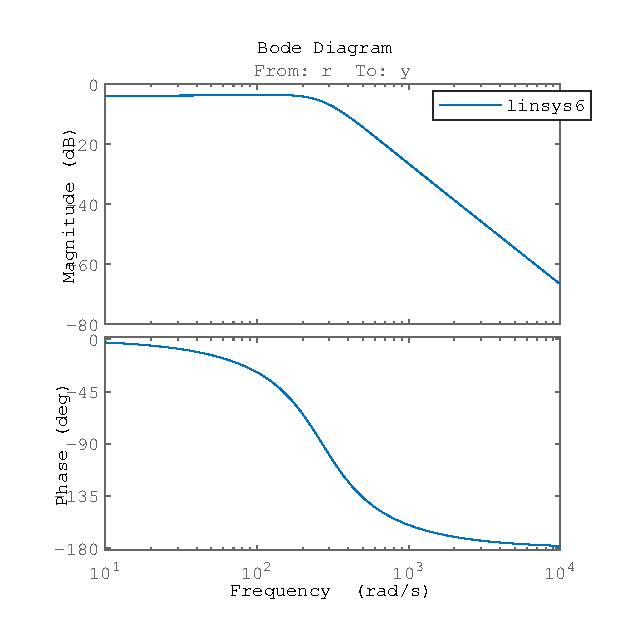
\includegraphics{images/Lab_2_Bode.eps}%
  }\hfill\\
  \subfloat[A much less damped, \(\zeta << 0.707,\) second order system.%
  \label{fig:lab2:bode:b}]{%
    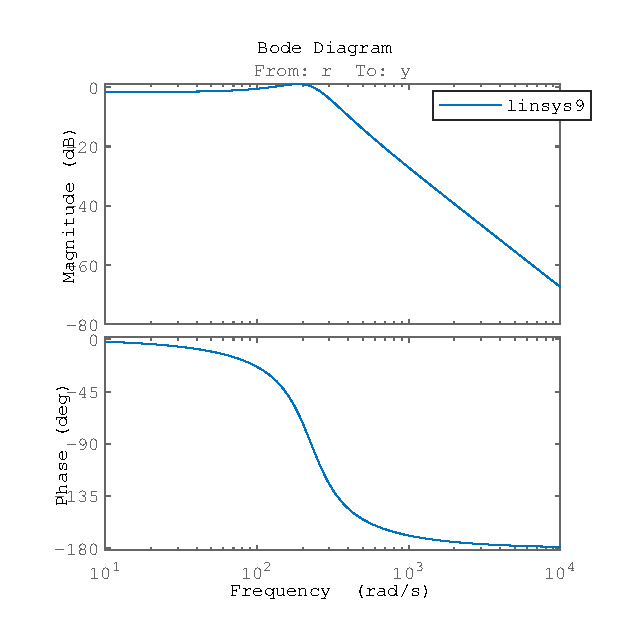
\includegraphics{images/Lab_2_Bode_Peak.eps}%
  }\hfill\\
  \caption[Sample Bode Plots of a Second Order System]{
    Sample Bode plots of a second order system.
  }
  \label{fig:lab2:bode}
\end{figure}
%
% \begin{figure}
%   \centering
%   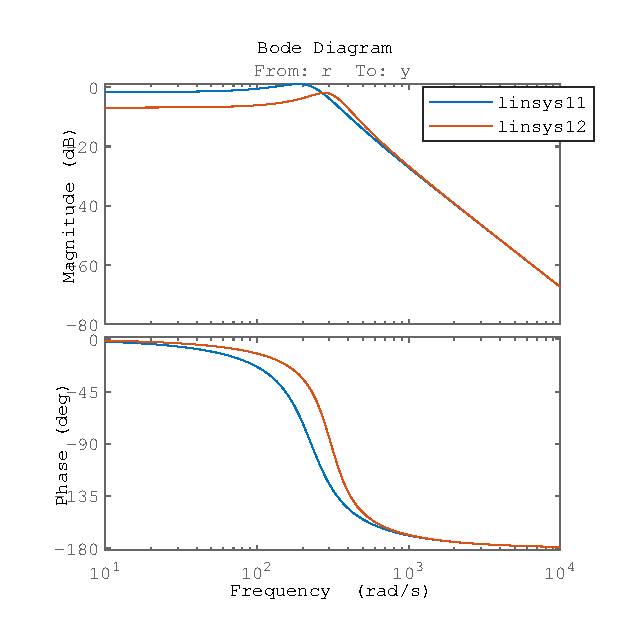
\includegraphics{images/Lab_2_Bode_ClosedLoop.eps}%
%   \caption[Sample Overlayed Bode Plots of a Second Order System]{
%     Sample overlayed Bode plots of a second order system.
%   }
%   \label{fig:lab2:bodeclosed}
% \end{figure}
%

\subsection{Disturbance Rejection}
You have almost completed the experimental part of this lab. This section
explores how the closed-loop affects disturbance rejection. Disturbances are
signals that we haven't modelled \emph{or} cannot be modelled and therefore
cannot account for. Naturally, large enough disturbances affect our ability to
control systems. The beauty of control is that we can design systems that
mitigate disturbances we do not explicitly model or know about! Here we will
find that our system can mitigate some types of disturbance signals, but not
all. The only deliverable for this section is
%
\begin{deliverable}[label={lab2:d4}]
  \textbf{Include} a Bode plot illustrating the response from the
  \emph{disturbance input signal} \(d(t)\) to the output signal \(y(t).\)
  \textbf{Include} a cursor on the magnitude plot at \emph{the bandwidth
  frequency of the closed loop system.} (The frequency found in
  Deliverable~\ref{lab2:d3})
\end{deliverable}
%
To fulfill this deliverable, you must acquire a Bode plot of the input to
output relationship between \(d\) and \(y.\)
%
\begin{procedure}[label={proc:lab2:p5}]
  For this procedure, you will change the input signal. You will remove the
  ``\texttt{Input Perturbation}'' annotation from the reference \(r\) and
  place it on the disturbance \(d.\)

  \begin{enumerate}[label=(\arabic*)]
    \item{
      \textbf{Ensure} the system is in the closed-loop configuration
      depicted in Figure~\ref{fig:lab2:closing-loop}.
      \textbf{Set} the gain \(K_p\) to \(1.\)
    }
    \item{
      \textbf{Remove} the ``\texttt{Input Perturbation}'' annotation from
      the reference signal. This amounts to repeating the process described
      in Appendix~\ref{App:Simulink:ModelLinearizer:2}, i.e. right click the
      signal wire \(r\) and press
      \texttt{Linear Analysis Points/Input Perturbation} so that the
      input perturbation icon disappears from the signal wire \(r.\)
    }
    \item{
      \textbf{Add} the ``\texttt{Input Perturbation}'' annotation to the
      the disturbance signal wire \(d.\)
    }
    \item{
      \textbf{Open} the Model Linearizer App and \textbf{acquire} a Bode
      plot. \emph{Expect the Bode plot to look substantially different than
      your previous Bode plots.}
    }
  \end{enumerate}
\end{procedure}

\section{Report Deliverable}
Good job! You made it through Lab~\ref{Lab:2}.
You are required to submit a report
that verifies you completed Lab~\ref{Lab:2} and that demonstrates you
understand the procedures you performed. In addition to including
\begin{itemize}
  \item{Deliverable~\ref{lab2:d1},}
  \item{Deliverable~\ref{lab2:d2},}
  \item{Deliverable~\ref{lab2:d2b},}
  \item{Deliverable~\ref{lab2:d3a},}
  \item{Deliverable~\ref{lab2:d3} and }
  \item{Deliverable~\ref{lab2:d4}}
\end{itemize}
in your report,
you are required to answer the questions of the following deliverable.
Make sure to leverage your other deliverables in your answers!
\begin{deliverable}[label={lab2:report}]
  \begin{enumerate}[label={(\arabic*)}]
    \item{
      Using the characteristics collected in Step~\ref{proc:lab2:p1:4} of
      Procedure~\ref{proc:lab2:p1}, \textbf{determine} the parameters
      \(\hat{K},\) \(\omega_n\) and \(\zeta\) that describe your plant \(P(s)\)
      in the standard second order form
      \[
        P(s) = \frac{\hat{K} \omega_n^2}{s^2 + 2 \zeta \omega_n s + \omega_n^2}
        .
      \]
      \emph{Notes: This time you drove the system with a unit
      step input. As a result, the steady-state value \(y_\mathrm{ss}\)
      is equal to the DC gain \(\hat{K}.\) The \(2\%\) settling time for a
      underdamped, standard second order system is approximated by the expression
      \[
        T_{2\%} \approx \frac{4}{\zeta \omega_n}
      \]
      and the percent overshoot is given by the formula
      \[
        \%\mathrm{OS} = 100 e^{\left(
          \frac{-\zeta \pi}{\sqrt{1-\zeta^2}}
        \right)}.
      \]
      So you should be able to solve for \(\hat{K}\) and \(\zeta\) first, then
      use them to solve for \(\omega_n.\)
      }
      \label{lab2:report:q1}
    }
    \item{
      It can be shown that the time-to-peak, another measurement you
      acquired, is equal to
      \[
        T_p = \frac{\pi}{\omega_n \sqrt{1-\zeta^2}}.
      \]
      Using your already acquired estimate of \(\zeta,\) \textbf{estimate}
      \(\omega_n\) using the time-to-peak.
      Based on your estimates, \textbf{explain} which you would rather use to
      estimate \(\omega_n:\) the time-to-peak or the \(2\%\) settling time.
      \label{lab2:report:q2}
    }
    \item{
      For the closed-loop diagram of Figure~\ref{fig:lab2:closing-loop},
      \textbf{compute} the transfer function from \(r\) to \(y.\)
      \textbf{Compute} the damping ratio, DC gain, and natural frequency of the
      closed-loop second-order system in terms of your plant's
      \(\hat{K},\) \(\omega_n\) and \(\zeta.\)
      \label{lab2:report:q3}
    }
    % \item{
    %   Given the open-loop damping ratio and natural frequency found in
    %   \ref{lab2:report:q1} and closed-loop damping ratio and natural
    %   frequency derived in~\ref{lab2:report:q2},
    %   \textbf{discuss} how closing the loop with unity feeback (\(K_p = 1\))
    %   affects the damping ratio and natural frequency of the
    %   second order system.
    %   \label{lab2:report:q3}
    % }
    \item{
      Using the table filled out in Deliverable~\ref{lab2:d2b} and the
      formulas you derived in~\ref{lab2:report:q3},
      \textbf{discuss} how changing the
      gain \(K_p\) affects the steady-state value \(y_\mathrm{ss},\) the
      time-to-peak \(T_p\) and the percent overshoot \(\%\mathrm{OS}.\)
      of the closed-loop second order step response.
      Also \textbf{discuss} how the settling time theoretically changes in the
      closed loop as a function of \(K_p\) using the estimate formula shown in
      \ref{lab2:report:q1}.
      \emph{\textbf{Ensure} you discuss every characteristic
      you've collected; if there is no trend, say so; if the trend is
      complicated (not simply linear in \(K_p\)), say so.}
      \label{lab2:report:q4}
    }
    \item{
      By leveraging your answer for~\ref{lab2:report:q4}, \textbf{explain} why
      proportional error feedback control may not always be sufficient to
      control a physical system.
      \label{lab2:report:q4b}
    }
    \item{
      Using the bandwidth frequencies found in Procedures~\ref{proc:lab2:p3}
      and~\ref{proc:lab2:p4}, \textbf{state} how closing the loop
      changed the bandwidth frequency.
      \label{lab2:report:q5}
    }
    % \item{
    %   \textbf{Why} is it desireable to be able to change the bandwidth
    %   of a system?
    %   \label{lab2:report:q7}
    % }
    \item{
      Leveraging Deliverable~\ref{lab2:d4}, \textbf{discuss} how well the
      closed loop system rejects disturbance signals.
      \emph{Your answer should depend on the disturbance input frequency
      \(\omega\) and the closed loop bandwidth frequency which you marked
      on your plot.}
      \label{lab2:report:q6}
    }
    % \item{
    %   For the open-loop configuration, \textbf{derive} the transfer function
    %   from the disturbance signal \(d\) to the output \(y.\)
    %   \textbf{Compare} the disturbance rejection properties between the
    %   open-loop and closed-loop system.
    %   \label{lab2:report:q7}
    % }
    \item{
      \textbf{Derive} the closed-loop transfer function from the
      disturbance \(d\) to the output \(y.\) How do the disturbance rejection
      properties change as you increase \(K_p\)? Do they improve or degrade?
      \emph{You will receive full marks if you provide a theoretical
      justification. You will want to produce a transfer function from
      \(d\) to \(y\) and it will have the form
      \[
        \frac{s^2 + A s + B}{s^2 + A s + D}
      \]
      where \(A, B, D\) depend on the plant parameters and \(K_p.\)
      \(K_p\) should only appear in \(D.\) You can then split the
      above system into two subsystems
      \[
        \left[s^2 + A s + B\right]
        \left[\frac{1}{D}\frac{D}{s^2 + A s + D}\right]
      \]
      and recognize that \(K_p\) only affects the Bode plot of the latter
      system. This means it suffices to analyze the frequency response of
      \[
        \frac{1}{D}\frac{D}{s^2 + A s + D}
      \]
      as \(K_p\) varies. You can put this subsystem into standard second order
      form to aid in your analysis. You already should be able to argue how the
      DC gain and natural frequency of this new subsystem is affected by
      \(K_p,\) so it remains to connect this knowledge with how the Bode plot
      of this subsystem would be affected.}

      \emph{An empirical argument (showing the Bode plot for multiple \(K_p\))
      will receive at most half the marks.}

      \emph{A correct answer without proof of any sort will receive 1 mark.}
      \label{lab2:report:q8}
    }
  \end{enumerate}
\end{deliverable}

\subsection{Grading Scheme}
The grading scheme is shown in Table~\ref{tab:lab2:grading}. The breakdown of
your grade is shown per deliverable except in the case of the lab
questions where it is shown per question.
%
\begin{table}
\centering
\begin{tabular}{c|l|c}
        & Deliverable           & Marks  \\ \hline
        & \ref{lab2:d1}         & 5       \\ \hline
        & \ref{lab2:d2}         & 5       \\ \hline
        & \ref{lab2:d3a}        & 5       \\ \hline
        & \ref{lab2:d3}         & 5       \\ \hline
        & \ref{lab2:d4}         & 5       \\ \hhline{=|=|=}
Lab Subtotal&                       & 25      \\ \hhline{=|=|=}
        & \ref{lab2:report}~\ref{lab2:report:q1}  & 3       \\ \hline
        & \ref{lab2:report}~\ref{lab2:report:q2}  & 2       \\ \hline
        & \ref{lab2:report}~\ref{lab2:report:q3}  & 3       \\ \hline
        & \ref{lab2:report}~\ref{lab2:report:q4}  & 4       \\ \hline
        & \ref{lab2:report}~\ref{lab2:report:q4b} & 1       \\ \hline
        & \ref{lab2:report}~\ref{lab2:report:q5}  & 1      \\ \hline
        & \ref{lab2:report}~\ref{lab2:report:q6}  & 3      \\ \hline
        & \ref{lab2:report}~\ref{lab2:report:q8}  & 4       \\ \hhline{=|=|=}
Report Subtotal&  & 21 \\ \hhline{=|=|=}
  Total &                       & 46
\end{tabular}
\caption[Grading Scheme for Lab 2]{Grading scheme for Lab 2.}
\label{tab:lab2:grading}
\end{table}
%

\chapter{Bringing it Together: Lateral Motion Control}\label{Lab:3}
Imagine you are a young, aspiring, junior engineer at VenX, a private company in an alternate Universe, manufucturing a mining probe on Venus%
\footnote{This society isn't particularly concerned about the environmental impact. It isn't our planet, right?}.
Because of your junior status, they have only asked you to design a simple controller that ensures the lunar module lands at the correct location.
The controller you design controls the level of horizontal thrust to achieve a desired position relative to some point on the surface.
You may assume that all units are in standard units.
Distances are measured in meters, time is measured in seconds, mass is measured in kilograms and all other units are such that they are consistent with that.

\section{Objectives}
\begin{enumerate}[label=(\arabic*)]
  \item{
    \textbf{Use} the skills you learned in Labs~\ref{Lab:1} and~\ref{Lab:2}
    to identify parameters of an opaque, black box system.
  }
  \item{
    \textbf{Design} a proportional inner-loop controller that stabilizes the velocity and controls it to a desired value.
  }
  \item{
    \textbf{Design} a proportional outer-loop controller that stabilizes the relative position of the lunar module with respect to a set point on the ground.
  }
  \item{
    \textbf{Derive} a mathematical expression for your controller and use this to \textbf{achieve} a desired control objective.
  }
  \item{
    \textbf{Compare and contrast} your stabilizing control design with that of Lab~\ref{Lab:2}.
  }
  \item{
    \textbf{Appreciate} how your controller deals with disturbances and unmodelled dynamics.
  }
\end{enumerate}

\section{Experimental Procedure}\label{Lab:3:Experiment}
Unlike previous labs, you will now work with two Simulink models.
Moreover, this lab will involve a larger number of moving parts;
you will introduce three feedback interconnections!

In Section~\ref{Lab:3:Part:I} you will stabilize the physical plant that maps input forces to an output horizontal velocity.
You will treat velocity as the measurement (output).
You can then design a controller

\subsection{Part I: Stabilize and Identify the Plant}\label{Lab:3:Part:I}
Your deliverables for this subsection are
%
\begin{deliverable}[label={del:lab3:g1:1}]
  \textbf{Choose} and \textbf{record} a gain value \(K_1\) for your stabilizing gain.
\end{deliverable}
%
\begin{deliverable}[label={del:lab3:g1:2}]
   \textbf{Acquire} the step response from the signal labelled \(w(t)\) to the signal \(v(t)\) when the signal \(v(t)\) is connected to the \(G_1\) loop summing junction (aptly named ``\(G_1\) Loop'').
\end{deliverable}
%
\begin{deliverable}[label={del:lab3:g1:3}]
  \textbf{Measure} the time constant \(\tau_1\) of your stabilized plant using the step response acquired in Deliverable~\ref{del:lab3:g1:2}.
\end{deliverable}
%
This section concerns the Part I area of the Simulink model
\begin{center}
  \texttt{Lab\_3\_Velocity\_Controlled\_Landing\_Module.slx}.
\end{center}
In this lab, your plant is a simulated physical system.
The system has nonlinear dynamics, but we will treat it as a linear system and you will observe the power of linear control.
First, in order to even design a controller to achieve our objectives, we must stabilize the system.
The reason for this is quite simple. A physical system normally integrates the input force into velocity (and then position) and, unless there are external forces such as friction, the plant is of the form
\[
  P(s)
    =
      \frac{1}{M s}
\]
where \(M > 0\) is the mass of the landing module.
The step response of this system is unbounded.
It is true that there is friction in your model but it is often hard to model friction in reality, so we will take the above equation as our model.
To stabilize the plant, consider closing the loop in the following way
%
\begin{center}
  \begin{tikzpicture}[x=1in, y=1in]

    \node [draw, smooth_block] (Plant) {\(P(s)\)};
    \node [draw, smooth_block, left = 0.75 of Plant] (Gain1) {\(K_1\)};
    \node [draw, smooth_sum, left = 0.75 of Gain1] (Sum1) {};
    \node [right = 0.75 of Plant] (after_plant) {};
    \node [right = 0.75 of after_plant] (v) {};
    \node [left = 0.75 of Sum1] (w) {};

    \node [smooth_annotate, below = 0 of Gain1] {Stabilizing Gain};
    \node [smooth_annotate, below = 0 of Plant] {Plant};

    \draw [arrow, smooth_path]
      (Plant.east) -- (after_plant.base) -- (v.base);
    \draw [arrow, smooth_path]
      (Plant.east)
      --
      (after_plant.base)
      --
      +(0, -0.75)
      -|
      (Sum1.south)
      node [below right] {\(-\)};
    \draw [arrow, smooth_path]
      (Sum1.east)
      --
      (Gain1.west);
    \draw [arrow, smooth_path]
      (Gain1.east)
      --
      (Plant.west);
    \draw [arrow, smooth_path]
      (w.base)
      --
      (Sum1.west);
  \end{tikzpicture}
\end{center}
%
with a randomly chosen gain \(K_1 > 0.\)
The gain you choose is up to you but make sure you record it.
\begin{procedure}[label={proc:lab3:stabilize}]
  This procedure simply reiterates the steps above.
  \begin{enumerate}[label={(\arabic*)}]
    \item{%
      \textbf{Close} the loop as described above.
      You should connect the signal labelled \(v\) to the summing junction labelled ``\(G_1\) Loop.''%
    }
    \item{%
      \textbf{Choose} and \textbf{set} a random positive gain for \(K_1.\)
      The block is named ``Stabilizing Gain'' in the Simulink model.%
    }
    \item{%
      \textbf{Acquire} a step response from the signal \(w(t)\) to the signal \(v(t).\)
      Remember from Lab 2 that you need to set \(w\) as an input perturbation and \(v\) as an output measurement.
    }
    \item{%
      \textbf{Measure} the time constant of this system using the acquired step response. We will call this time constant \(\tau_1.\)
    }
  \end{enumerate}
\end{procedure}

\subsection{Part II: Reference Velocity Control Design}\label{Lab:3:Part:II}
When you performed Procedure~\ref{proc:lab3:stabilize}, you will have noticed that the step response was extremely slow.
In particular, you should notice that it took more than a minute of simulated time to achieve a speed of \SI{1}{m/s} (\SI{3.6}{km/h})!
If this is the response speed of our system, we will never be able to control it to a desired position.
In this section, you will solve this problem by designing a proportional error feedback controller that controls to a \emph{desired velocity} but with a much better time constant.
Your deliverables for this section are
%
\begin{deliverable}[label={del:lab3:g2:1}]
  \textbf{Acquire} a (unit) step response from the signal \(v_r(t)\) to the signal \(v(t).\)
  \textbf{Ensure} you have cursors that indicate the following:
  \begin{itemize}
    \item{the time constant is \(\frac{1}{\sqrt{50}} \approx 0.1414.\)}
    \item{the DC gain, or steady-state value, is \(1.\)}
  \end{itemize}
\end{deliverable}
%
This section concerns the Part II area of the Simulink model
\begin{center}
  \texttt{Lab\_3\_Velocity\_Controlled\_Landing\_Module.slx}.
\end{center}
The now stabilized plant, as a transfer function from \(w(t)\) to \(v(t),\) will be referred to as \(G_1(s)\) as is depicted below.
Verify for yourself that
\[
  G_1(s) = \frac{1}{\tau_1 s + 1}
\]
where \(\tau\) is the time constant of \(G_1(s)\) (as estimated in Deliverable~\ref{del:lab3:g1:timeconstant}).
Close the loop around \(G_1(s)\) with a proportional error feedback controller like so
%
\begin{center}
  \begin{tikzpicture}[x=1in, y=1in]

    \node [draw, smooth_block] (Plant) {\(P(s)\)};
    \node [draw, smooth_block, left = 0.25 of Plant] (Gain1) {\(K_1\)};
    \node [draw, smooth_sum, left = 0.25 of Gain1] (Sum1) {};
    \node [right = 0.25 of Plant] (after_plant) {};
    \node [right = 0.50 of after_plant] (v) {};
    \node [left = 0.50 of Sum1] (w) {};

    \draw [arrow, smooth_path]
      (Plant.east) -- (after_plant.base) -- (v.base)
      node [above right] {\(v(t)\)};
    \draw [arrow, smooth_path]
      (Plant.east)
      --
      (after_plant.base)
      --
      +(0, -0.50)
      -|
      (Sum1.south)
      node [below right] {\(-\)};
    \draw [arrow, smooth_path]
      (Sum1.east)
      --
      (Gain1.west);
    \draw [arrow, smooth_path]
      (Gain1.east)
      --
      (Plant.west);
    % \draw [arrow, smooth_path]
    %   (w.base)
    %   --
    %   (Sum1.west);

    \draw [smooth_area_path, fill = Blue, fill opacity = 0.50, text opacity = 1]
      ($(w)+(0.25, 0)$) -- +(0, 0.50) -| node[midway, above, color=Blue] {\(G_1(s)\)} ($(v)+(-0.50,0)$) -- +(0, -0.75) -| ($(w)+(0.25, 0)$);

    \node [draw, smooth_block, left = 0.25 of w] (Gain2) {\(K_2\)};
    \node [draw, smooth_sum, left = 0.50 of Gain2] (Sum2) {};
    \node [left = 0.50 of Sum2] (v_r) {};

    \draw [arrow, smooth_path]
      (Plant.east)
      --
      ($(v)+(-0.25,0)$)
      --
      +(0, -1)
      -|
      (Sum2.south)
      node [below right] {\(-\)};
    \draw [arrow, smooth_path]
      (Sum2.east)
      --
      (Gain2.west);
    \draw [arrow, smooth_path]
      (Gain2.east)
      --
      (Sum1.west);
    \draw [arrow, smooth_path]
      (v_r.base)
      --
      (Sum2.west)
      node [midway, above] {\(v_r(t)\)};

  \end{tikzpicture}
\end{center}
%
Verify that, when the loop is closed, the transfer function from \(v_r(t)\) to \(v(t),\) denoted as \(G_2(s)\) in the Simulink model, takes the form
\[
  G_2(s)
    = \frac{V(s)}{V_r(s)}
    = \frac{K_3 K_2}{1 + K_2} \frac{1}{\frac{\tau_1}{1 + K_2} s + 1}.
\]
%
\begin{procedure}[label={proc:lab3:speedup}]
  In this procedure you use another closed loop to accelerate the response of your system, thereby making it usable to do position step tracking.
  \begin{enumerate}[label={(\arabic*)}]
    \item{%
      \textbf{Close} the loop as described above.
      You should connect the signal labelled \(v\) to the summing junction labelled ``\(G_2\) Loop.''%
    }
    \item{%
      We would like to have the transfer function \(G_2(s)\) to have a time constant of \(\frac{1}{\sqrt{50}}.\)
      This would mean that, for a step change in the \emph{reference velocity}, the \emph{actual velocity} will reach \(63.3\%\) of the reference velocity in \SI{0.1414}{s}.
      Recognize that the time constant of this new closed loop system is
      \[
        \frac{\tau_1}{1 + K_2}
      \]
      where \(\tau_1\) is the time constant of \(G_1(s)\) that you measured earlier.
      As a result, \textbf{solve} for the \(K_2\) you need to have this time constant equal to \(\frac{1}{\sqrt{50}}.\)%
    }
    \item{%
      \textbf{Solve} for the gain \(K_3\) that ensures \(G_2(s)\) has a DC gain of \(1.\)%
    }
    \item{%
      \textbf{Set} the respective blocks corresponding to \(K_2\) and \(K_3\) in the Simulink diagram.%
    }
    \item{%
      \textbf{Acquire} the step response from the signal \(v_r(t)\) to the signal \(v(t).\)
      Remember again to change which signal is the input perturbation from Part I.%
    }
    \item{%
      \textbf{Place} cursors on the time constant and steady-state value to prove you met the specification.%
    }
  \end{enumerate}
\end{procedure}

\subsection{Part III: Reference Position Control Design}\label{Lab:3:Part:III}
Your deliverables for this part are
%
\begin{deliverable}[label={del:lab3:g3:1}]
   \textbf{Acquire} the step response from the signal labelled \(r(t)\) to the signal \(x(t)\) when the signal \(x(t)\) is connected to the \(G_3\) loop summing junction (aptly named ``\(G_3\) Loop'').
   This is the step response of the transfer function \(G_3(s)\) depicted in the Simulink model.
\end{deliverable}
%
\begin{deliverable}[label={del:lab3:g3:2}]
   \textbf{Run} the ``\texttt{visualize\_landing.m}'' script and \textbf{save} both Figures that are generated.
\end{deliverable}
%
\begin{deliverable}[label={del:lab3:g3:3}]
   \textbf{Acquire} the Bode plot from the signal labelled \(d(t)\) to the signal \(x(t).\)
\end{deliverable}
%
This section concerns the Part III area of the Simulink model
\begin{center}
  \texttt{Lab\_3\_Position\_Controlled\_Landing\_Module.slx}.
\end{center}
You will notice that the other Simulink model you worked with is labelled \(G_2(s)\) in this model.
Since you have designed a controller that achieves a desired reference velocity, we leverage it in this model to design an outer loop controller that achieves a desired position.
Close the loop to arrive at a diagram
%
\begin{center}
  \begin{tikzpicture}[x=1in, y=1in]

    \node [draw, smooth_block] (G2) {\(G_2(s)\)};
    \node [draw, smooth_block, right = 0.75 of G2] (Int) {\(\frac{1}{s}\)};
    \node [draw, smooth_block, left = 0.75 of G2] (Gain4) {\(K_4\)};
    \node [draw, smooth_sum, left = 0.75 of Gain4] (Sum3) {};
    \node [right = 0.25 of Int] (after_int) {};
    \node [right = 0.50 of after_int] (x) {};
    \node [left = 0.50 of Sum3] (r) {};

    \draw [arrow, smooth_path]
      (G2.east) -- (Int.west)
      node [above, midway] {\(v(t)\)};
    \draw [arrow, smooth_path]
      (Int.east) -- (after_int.base) -- (x.base)
      node [above] {\(x(t)\)};
    \draw [arrow, smooth_path]
      (Int.east)
      --
      (after_int.base)
      --
      +(0, -0.50)
      -|
      (Sum3.south)
      node [below right] {\(-\)};
    \draw [arrow, smooth_path]
      (Sum3.east)
      --
      (Gain4.west);
    \draw [arrow, smooth_path]
      (Gain4.east)
      --
      (G2.west);
    % \draw [arrow, smooth_path]
    %   (w.base)
    %   --
    %   (Sum1.west);

    \draw [arrow, smooth_path]
      (r.base)
      --
      (Sum3.west)
      node [midway, above] {\(r(t)\)};

  \end{tikzpicture}
\end{center}
%
If you performed Part II correctly, the transfer function \(G_2(s)\) takes the
form
\[
  G_2(s) = \frac{1}{\frac{1}{\sqrt{50}}s + 1}.
\]
Verify that the transfer function from \(r(t)\) to \(x(t),\) denoted \(G_3(s)\) in the Simulink model, equals
\[
  G_3(s) = \frac{K_4\sqrt{50}}{s^2 + \sqrt{50} s + K_4 \sqrt{50}}.
\]
%
\begin{procedure}[label={proc:lab3:regulate}]
  You will make a specific choice for \(K_4\) in this procedure and then simulate the entire non-linear system.
  \begin{enumerate}[label={(\arabic*)}]
    \item{%
      \textbf{Close} the loop as described above.
      You should connect the signal \(x(t)\) to the \(G_3\) loop summing junction (aptly named ``\(G_3\) loop'').%
    }
    \item{%
      \textbf{Determine} and \textbf{set} the gain \(K_4\) so that the system \(G_3(s)\) is critically damped.
      To be clear, with your choice of \(K_4\) you should find that \(\zeta = 1\) when \(G_3(s)\) is put in standard form.%
    }
    \item{%
      \textbf{Acquire} the (unit) step response from the signal \(r(t)\) to the signal \(x(t).\)
      Remember to go into the other model file and remove any annotations you have used there before setting new ones in this model file.%
    }
    \item{%
      \textbf{Run} the ``\texttt{visualize\_landing.m}'' script and \textbf{save} both Figures that are generated.%
      \emph{Do not be alarmed that the behaviour does not look like the step response.}
    }
  \end{enumerate}
\end{procedure}
%
In the following procedure, be very careful where you place your annotations, and make sure to save your diagram before running the Model Linearizer.
You must complete the previous procedure before starting this final procedure.
%
\begin{procedure}[label={proc:lab3:disturbance}]
  In this procedure, you will acquire the Bode plot from the input force \(u(t)\) to the output position \(x(t).\)
  \begin{enumerate}[label={(\arabic*)}]
    \item{%
      \textbf{Ensure} you completed Procedure~\ref{proc:lab3:regulate}.
    }
    \item{%
      \textbf{Remove} all annotations from all signals in \emph{both} Simulink models.
    }
    \item{%
      \textbf{Set} the input perturbation annotation for the signal \(d(t)\) that is added into the signal right before the Plant block.
      \(d(t)\) is the signal coming out of the ``Disturbance Signal'' block.
    }
    \item{%
      \textbf{Set} the output measurement annotation for the signal \(x(t)\) right after the integrator block (found in the ``Position'' Simulink model).
    }
    \item{%
      \textbf{Acquire} the Bode plot.
    }
  \end{enumerate}
\end{procedure}
%

\section{Report Deliverable}
Wow you made it through the Lab 3 experiment! Good job! As usual, you are expected to submit a report demonstrating that you completed the lab and that you understand the tasks performed.
In addition to including
\begin{itemize}
  \item{Deliverable~\ref{del:lab3:g1:1},}
  \item{Deliverable~\ref{del:lab3:g1:2},}
  \item{Deliverable~\ref{del:lab3:g1:3},}
  \item{Deliverable~\ref{del:lab3:g2:1},}
  \item{Deliverable~\ref{del:lab3:g3:1},}
  \item{Deliverable~\ref{del:lab3:g3:2} and}
  \item{Deliverable~\ref{del:lab3:g3:3}}
\end{itemize}
in your report, you are required to answer the questions of the following deliverable.
Make sure to leverage your other deliverables in your answers!
\begin{deliverable}[label={lab3:report}]
  \begin{enumerate}[label={(\arabic*)}]
    \item{%
      The entire closed loop system \(G_3(s)\) can be described by the diagram in Figure~\ref{fig:lab3:entire}.
      \textbf{Derive} the transfer function from \(r(t)\) to \(x(t)\)
      in terms of the \emph{symbols} \(K_1,\) \(K_2,\) \(K_3,\) \(K_4,\) and \(M.\)
      Leave your answer in symbolic form.
      \emph{It is not required, but it is wise to verify your answer against the transfer functions discussed throughout the lab. They should be consistent.}
      \label{lab3:report:q1}
    }
    \item{%
      You should find that the transfer function that you derived in~\ref{lab3:report:q2} was a second-order transfer function with no zero.
      \textbf{Write} the transfer function of~\ref{lab3:report:q2} in standard second order form by deducing what its DC gain \(\hat{K},\) natural frequency \(\omega_n\) and damping ratio \(\zeta\) are in terms of the symbols \(K_1,\) \(K_2,\) \(K_3,\) \(K_4,\) and \(M.\)
      Leave your answer in symbolic form.
      \label{lab3:report:q2}
    }
    \item{%
      Unlike in Lab 2, you can change the settling time of the final, second order transfer function from \(r(t)\) to \(y(t).\)
      Leveraging the formula that estimates the \(2\%\) settling time
      \[
        T_{2\%} \approx \frac{4}{\zeta \omega}
      \]
      for a transfer function in standard form \textbf{identify} the two gains that affect the settling time of your transfer function \(G_3(s)\) (use the standard form derived in~\ref{lab3:report:q2}) .
      \label{lab3:report:q3}
    }
    \item{%
      To produce Deliverable~\ref{del:lab3:g3:2}, you simulated the true response of your controller against the complete, nonlinear system;
      not a linear approximation of it!
      The Model Linearizer performs a linear approximation of the nonlinear differential equation found in the Plant block.
      It then gives you the step response of the corresponding linear system's transfer function.
      As a result, you designed against only an approximation of the true system.
      This explains why you will have observed a modest to large overshoot of the target horizontal position before the landing module settles.
      That doesn't mean linear system theory is completely useless, however.
      \textbf{Determine} a gain that you can change to reduce the overshoot.
      \textbf{Justify} your explanation using your solution to~\ref{lab3:report:q2} and make sure to include whether you would increase or decrease that gain.
      \emph{It is not required, but I highly recommend you give it a try and see if it works. You might be surprised!}
      \label{lab3:report:q4}
    }
    \item{%
      As mentioned in~\ref{lab3:report:q5}, to produce Deliverable~\ref{del:lab3:g3:2} you simulated your control design against the real system.
      The engineers at VenX included in that model a wind force, that increases in magnitude as you get closer to the ground \emph{and} has some sinusoidal variability in speed.
      As part of the specification, the engineers would like to know just how large of a force we can afford.

      Since wind is just an additional force, and \(u(t)\) is really just an input force, we can model this wind force as simply an additional signal \(d(t)\) that is added to the input of the Plant \(u(t).\)
      Assume
      \[
        d(t) = M + A\sin\left(\pi t\right),
      \]
      where \(M, A > 0\).
      Using the Bode plot you acquired in Deliverable~\ref{del:lab3:g3:3},
      \textbf{justify} why you did not notice this sinusoidal force in your response acquired in Deliverable~\ref{del:lab3:g3:2}.
      \textbf{Specifically determine} how large \(A\) would have to be to observe a sinusoid of amplitude \SI{1}{m} in the output.
      \label{lab3:report:q5}
    }
    \item{%
      The software developers at VenX want your controller to have \(x(t),\) your horizontal position, to track perfectly any constant reference position \(r(t).\)

      Does your control system (treating \(r(t)\) as the input and \(x(t)\) as the output) do this?
      If yes, does it matter what the constants \(K_1,\) \(K_2,\) \(K_3,\) \(K_4,\) and \(M\) are?
      \textbf{Justify} using the theory learned in the course.
      \emph{Use the transfer function \(G_3(s)\) put in standard form (as derived in~\ref{lab3:report:q3}) to answer the question.}
      \label{lab3:report:q6}
    }
    \item{%
      The philosophy of this control design was to (1) design a controller that regulates a desired velocity fast enough by controlling the input force and (2) design a controller that regulates a desired position by controlling the desired velocity.
      This is a very common technique used in aerospace since it breaks the control design into smaller, easier chunks that aim to solve different problems.
      With this philosophy in mind, the data you have at hand, and the answers to all the previous questions, answer the following question as best as you possibly can:

      Your supervisor at the company VenX was alarmed by your Deliverable~\ref{del:lab3:g3:2}.
      They think the acceleration imparted by your controller is too large and could damage delicate components that are deployed on descent.
      How could you decrease the acceleration imparted by your controllers?
      \label{lab3:report:q7}
    }
  \end{enumerate}
\end{deliverable}

\begin{figure}
  \centering
  \begin{tikzpicture}[x=1in, y=1in]
    \node[smooth_block] (Plant) {\(\frac{K_1}{M s}\)};
    \node[smooth_sum, left = 0.3 of Plant] (Sum1) {};
    \node[smooth_block, left = 0.3 of Sum1] (K2) {\(K_2\)};
    \node[smooth_sum, left = 0.3 of K2] (Sum2) {};
    \node[smooth_block, left = 0.3 of Sum2] (K3K4) {\(K_4 K_3\)};
    \node[smooth_sum, left = 0.3 of K3K4] (Sum3) {};
    \node[left = 0.3 of Sum3] (r) {};
    \node[right = 0.3 of Plant] (afterPlant) {};
    \node[smooth_block, right = 0.3 of afterPlant] (Int) {\(\frac{1}{s}\)};
    \node[right = 0.3 of Int] (afterInt) {};
    \node[right = 0.3 of afterInt] (y) {};

    \draw[smooth_path, arrow]
      (r.base)
      node[above] {\(r(t)\)}
      --
      (Sum3.west);
    \draw[smooth_path, arrow]
      (Sum3.east)
      --
      (K3K4.west);
    \draw[smooth_path, arrow]
      (K3K4.east)
      --
      (Sum2.west);
    \draw[smooth_path, arrow]
      (Sum2.east)
      --
      (K2.west);
    \draw[smooth_path, arrow]
      (K2.east)
      --
      (Sum1.west);
    \draw[smooth_path, arrow]
      (Sum1.east)
      --
      (Plant.west);
    \draw[smooth_path, arrow]
      (Plant.east)
      --
      (afterPlant.base)
      --
      (Int.west);
    \draw[smooth_path, arrow]
      (Int.east)
      --
      (afterInt.base)
      --
      (y.base)
      node[above] {\(y(t)\)};
    \draw[smooth_path, arrow]
      (Int.east)
      --
      (afterInt.base)
      --
      +(0, -1)
      -|
      (Sum3.south);
    \draw[smooth_path, arrow]
      (Plant.east)
      --
      (afterPlant.base)
      --
      +(0, -0.50)
      -|
      (Sum1.south)
      node[below right] {\(-\)};
    \draw[smooth_path, arrow]
      (Plant.east)
      --
      (afterPlant.base)
      --
      +(0, -0.75)
      -|
      (Sum2.south)
      node[below right] {\(-\)};

  \end{tikzpicture}
  \caption[Closed Loop system for Lab 3]{Entire closed loop architecture for Lab 3.}
  \label{fig:lab3:entire}
\end{figure}

\subsection{Grading Scheme}
The grading scheme is shown in Table~\ref{tab:lab3:grading}. The breakdown of
your grade is shown per deliverable except in the case of the lab
questions where it is shown per question.
%
\begin{table}
\centering
\begin{tabular}{c|l|c}
        & Deliverable           & Marks  \\ \hline
        & \ref{del:lab3:g1:1}         & 4       \\ \hline
        & \ref{del:lab3:g1:2}         & 4      \\ \hline
        & \ref{del:lab3:g1:3}        & 4       \\ \hline
        & \ref{del:lab3:g2:1}        & 4       \\ \hline
        & \ref{del:lab3:g3:1}         & 4      \\ \hline
        & \ref{del:lab3:g3:2}         & 4       \\ \hline
        & \ref{del:lab3:g3:3}         & 4       \\ \hhline{=|=|=}
Lab Subtotal&                       & 28      \\ \hhline{=|=|=}
        & \ref{lab3:report}~\ref{lab3:report:q1}  & 4       \\ \hline
        & \ref{lab3:report}~\ref{lab3:report:q2}  & 4       \\ \hline
        & \ref{lab3:report}~\ref{lab3:report:q3}  & 4       \\ \hline
        & \ref{lab3:report}~\ref{lab3:report:q4}  & 4       \\ \hline
        & \ref{lab3:report}~\ref{lab3:report:q5}  & 3      \\ \hline
        & \ref{lab3:report}~\ref{lab3:report:q6}  & 3      \\ \hline
        & \ref{lab3:report}~\ref{lab3:report:q7}  & 3      \\ \hhline{=|=|=}
Report Subtotal&  & 25 \\ \hhline{=|=|=}
  Total &                       & 53
\end{tabular}
\caption[Grading Scheme for Lab 3]{Grading scheme for Lab 3.}
\label{tab:lab3:grading}
\end{table}
%


%%%%%%%%%%%%%%%%%%%%%%%%%%%%%%%%%%%%%%%%%%%%%%%%%%%%%%%%%%%%%%%%%%%%%%%%%%%%%%%
% BEG: APPENDIX

\appendix
\chapter{On Simulink}\label{App:Simulink}

\section{Model Linearizer Tools}\label{App:Simulink:ModelLinearizer}
The model linearizer tools is an ``App'' in Simulink that allows an engineer to
(1) linearize a system and (2) perform linear system analyses such as Bode
plots and Step Responses. We won't be needing the first feature since our
systems are already linear. This section is a brief tutorial on how to use
the tools to acquire step responses, Bode plots and Nyquist plots.

\subsection{The Model Linearizer App}
To open the Model Linearizer App, look to the top of your Simulink Model
window and click the ``\texttt{APPS}'' button like so
%
\begin{center}
  \includegraphics[width=0.8\linewidth]{%
    app-model-linearizer-open-1.png%
  }
\end{center}
%
Then proceed to opening the application by clicking the ``\texttt{Model
Linearizer}'' button
%
\begin{center}
  \includegraphics[width=0.8\linewidth]{%
    app-model-linearizer-open-2a.png%
  }
\end{center}
%
If you cannot find it located in the toolbar depicted above, press the
dropdown on the far right of the toolbar
%
\begin{center}
  \includegraphics[width=0.8\linewidth]{%
    app-model-linearizer-open-2b.png%
  }
\end{center}
%
to view a larger list of options.
If you still cannot find it, you must not have the \texttt{Simulink Control Design} toolbox installed. Ensure you've installed the toolboxes listed in the
Introduction. Upon opening the Model Linearizer app, you
will have a window that looks like Figure~\ref{fig:app1:model-linearizer}.
%
\begin{figure}[H]
  \centering
  \includegraphics[width=0.8\linewidth]{%
    app-model-linearizer-opened.png%
  }
  \caption[The Model Linearizer App]{%
    What the Model Linearizer application looks like when you first open it.%
  }
  \label{fig:app1:model-linearizer}
\end{figure}

\subsection{Setting up your System: Input to Output}
\label{App:Simulink:ModelLinearizer:2}
Now that you know how to open up the Model Linearizer, we must prepare
the system we want to analyze. The Model Linearizer tool doesn't know what
we consider an ``input'' and what we consider an ``output'' just from our
Simulink diagram. But you do! Whenever you want to take a step response, you
know where you input the step and what measurements you want to observe.
The goal of the following steps is to show you how to give the Model
Linearizer App this information.

First pull up the Simulink model of concern. I'll use the Lab 1 diagram as
an example,
%
\begin{center}
  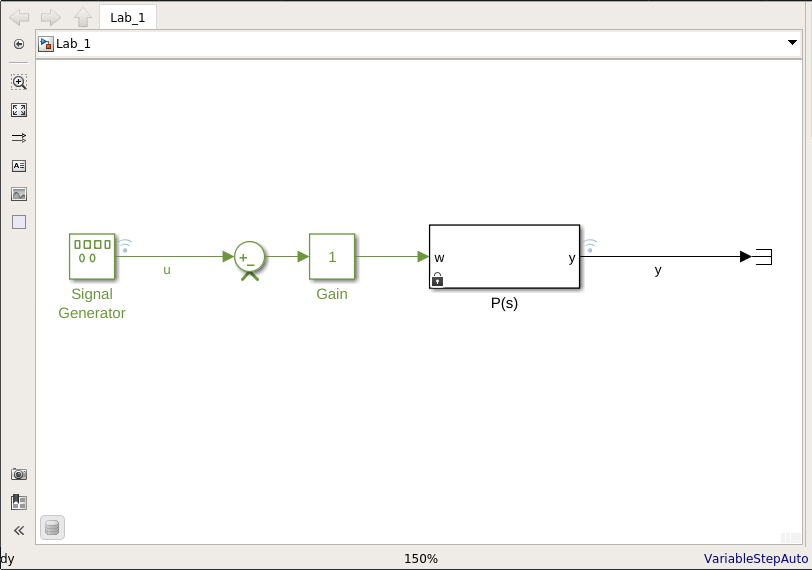
\includegraphics[width=0.8\linewidth]{app-model-linearizer-io-1.png}
\end{center}
%
Suppose we wanted to analyze the relationship between the signals
labelled \(u\) and \(y.\)
Right-click the signal wire labelled \(u\) and hover over ``Linear Analysis
Points'' as depicted in Figure~\ref{fig:app1:io-menu:a}.
%
\begin{figure}
  \centering
  \includegraphics[width=0.8\linewidth]{%
    app-model-linearizer-io-2a.png%
  }
  \caption{Signal context menu and Linear Analysis points submenu.}
  \label{fig:app1:io-menu:a}
\end{figure}
%
\begin{figure}
  \centering
  \includegraphics[width=0.8\linewidth]{%
    app-model-linearizer-io-2b.png%
  }
  \caption{The Linear Analysis context submenu.}
  \label{fig:app1:io-menu:b}
\end{figure}
%
This context menu has a number of options of which we will only use two.
Since we would like to indicate to the Model Linearizer App that this wire
is where the input appears, we select ``\texttt{Input Perturbation}.'' We
repeat the \emph{same exact} process for the desired output signal wire \(y\)
except we select ``\texttt{Output Measurement}.'' The result is
depicted in Figure~\ref{fig:app1:io-signals}. \emph{Note the little annotations
above the signal.}
A ``down'' arrow denotes an input and an ``up'' arrow denotes an output signal.
%
\begin{figure}
  \centering
  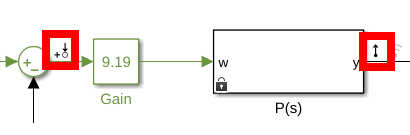
\includegraphics[width=0.8\linewidth]{app-model-linearizer-io-3.png}
  \caption{%
    The result after setting up an input signal and output
    measurement signal.%
  }
  \label{fig:app1:io-signals}
\end{figure}
%
You will have to repeat this process whenever you want to change where you
apply your input or when you want to observe a different output. Note that
the placement of the ``\texttt{Input Perturbation}'' and
``\texttt{Output Measurement}'' annotations is not arbitrary;
it is intentional! This
allows us to quickly change the configuration of the system, closing the loop
for example, and get closed-loop measurements without having to change our
annotations!

\FloatBarrier
\subsection{Acquiring Plots}
\label{App:Simulink:ModelLinearizer:3}
Having indicated to the Model Linearizer app the input and output signal, you
are now ready to acquire a step response. Open the Model Linearizer. Look at
the top bar of the Model Linearizer and confirm that it looks as depicted below:
%
\begin{center}
  \includegraphics[width=0.8\linewidth]{%
    app-model-linearizer-toolbar.png%
  }
\end{center}
%
Try pressing the ``\texttt{Step Response}'' button! You should get a response
like that of Figure~\ref{fig:app1:stepresponse}. Great! Now try clicking
on a point of the curve. You will then get something we call a \textbf{data
tip} or \textbf{cursor}, shown in Figure~\ref{fig:app1:cursors}.
You can drag this cursor (the black dot) around to a specific point on the
curve, allowing you to get accurate readings. Use this feature!
%
Similarly, one can capture a Bode plot, as depicted in Figure
\ref{fig:app1:bodeplot}, by pressing the ``\texttt{Bode}'' button.

Now that we can acquire these plots, how do we \emph{save} them? Notice that
above every plot is a name. For example, Figure~\ref{fig:app1:bodeplot} is
in a tab named ``Bode Plot 1.'' With this selected, you will see in the top
bar a larger tab with the same name. This is depicted in Figure
\ref{fig:app1:capturefigure}. In that tab, you can then press
``\texttt{Print to Figure}.'' Upon doing so, you have a Matlab Figure pop-up,
which then gives you the option --- under \texttt{File/Save As} --- to
export a \texttt{.png} or other image file.
%
\begin{figure}
  \centering
  \includegraphics[width=0.8\linewidth]{%
    app-model-linearizer-stepresponse.png%
  }
  \caption[Capturing a Step Response in the Model Linearizer App]{%
    Capturing a step response in the Model Linearizer app.
  }
  \label{fig:app1:stepresponse}
\end{figure}
%
\begin{figure}
  \centering
  \includegraphics[width=0.8\linewidth]{%
    app-model-linearizer-cursors.png%
  }
  \caption[Data Tips in Matlab Figures]{%
    I put two data tips, one near the settling value and another at
    just over \(0.5\) in amplitude.
  }
  \label{fig:app1:cursors}
\end{figure}
%
\begin{figure}
  \centering
  \includegraphics[width=0.8\linewidth]{%
    app-model-linearizer-bodeplot.png%
  }
  \caption[Bode Plot captured in the Model Linearizer App]{%
    A bode plot captured in the Model Linearize app. Do you know what special
    points I've marked on the Bode plot? Name them. Why are they important?
  }
  \label{fig:app1:bodeplot}
\end{figure}
%
\begin{figure}
  \centering
  \includegraphics[width=0.8\linewidth]{%
    app-model-linearizer-capturefigure.png%
  }
  \caption[Acquiring a Figure in the Model Linearizer App]{%
    This screenshot depicts how to turn a data acquisition into a Matlab
    Figure.
  }
  \label{fig:app1:capturefigure}
\end{figure}
%


% END: APPENDIX
%%%%%%%%%%%%%%%%%%%%%%%%%%%%%%%%%%%%%%%%%%%%%%%%%%%%%%%%%%%%%%%%%%%%%%%%%%%%%%%

\backmatter
\end{document}
